\documentclass[10pt,spanish,aspectratio=1610]{beamer}
\usepackage[utf8]{inputenc}
\usepackage{amsmath}
\usepackage{graphicx}
\usepackage{amssymb}
\usepackage{multicol}
\usepackage{subfig}
\usepackage{fancyhdr}
\usepackage{pstricks}
\usepackage{color}
\usepackage[ruled]{algorithm2e}
\usepackage{listings}
\usepackage{xcolor}
\usepackage{gensymb}

\definecolor{graywhite}{rgb}{0.9529,0.9607,0.9686}
\definecolor{bluegray}{rgb}{0.6823, 0.7411, 0.8}
\definecolor{darkred}{rgb}{0.7372, 0.2392, 0.2392}
\definecolor{bluedark}{rgb}{0.294, 0.4705, 0.6407}
\definecolor{darkgreen}{rgb}{0.1764, 0.5294, 0.0901}
\lstset{
  backgroundcolor=\color{graywhite},   % choose the background color; you must add \usepackage{color} or \usepackage{xcolor}; should come as last argument
  basicstyle=\footnotesize,        % the size of the fonts that are used for the code
  breakatwhitespace=false,         % sets if automatic breaks should only happen at whitespace
  breaklines=true,                 % sets automatic line breaking
  captionpos=b,                    % sets the caption-position to bottom
  commentstyle=\color{darkgreen},    % comment style
  keepspaces=true,                 % keeps spaces in text, useful for keeping indentation of code (possibly needs columns=flexible)
  keywordstyle=\color{darkred},       % keyword style
  language=Octave,                 % the language of the code
  morekeywords={*,...},            % if you want to add more keywords to the set
  numbers=left,                    % where to put the line-numbers; possible values are (none, left, right)
  numbersep=7pt,                   % how far the line-numbers are from the code
  numberstyle=\tiny\color{bluedark}, % the style that is used for the line-numbers
  showspaces=false,                % show spaces everywhere adding particular underscores; it overrides 'showstringspaces'
  showstringspaces=false,          % underline spaces within strings only
  showtabs=false,                  % show tabs within strings adding particular underscores
  stepnumber=1,                    % the step between two line-numbers. If it's 1, each line will be numbered
  stringstyle=\color{bluedark},     % string literal style
  frame=single,
  rulecolor=\color{bluegray},
  tabsize=2,                   % sets default tabsize to 2 spaces
  xleftmargin=1cm,
  xrightmargin=0.5cm,
  framexleftmargin=0.5cm,
  extendedchars=true,
  literate={á}{{\'a}}1 {é}{{\'e}}1 {í}{{\'i}}1 {ó}{{\'o}}1 {ú}{{\'u}}1 {Á}{{\'A}}1 {É}{{\'E}}1 {Í}{{\'I}}1 {Ó}{{\'O}}1 {Ú}{{\'U}}1,
}

\DeclareMathOperator{\atantwo}{atan2}
\setbeamercolor{block title}{fg=white,bg=blue!70!black}
\setbeamercolor{block body}{fg=black, bg=blue!10!white}
\setbeamertemplate{blocks}[rounded][shadow=false]
\setbeamercovered{transparent}
\beamertemplatenavigationsymbolsempty
\setbeamertemplate{frametitle}{
  \leavevmode
  \hbox{\begin{beamercolorbox}[wd=0.85\paperwidth,left]{frametitle}
    \usebeamerfont{frametitle}\insertframetitle
  \end{beamercolorbox}
%  \begin{beamercolorbox}[wd=0.25\paperwidth,center]{frametitle}
%    \usebeamerfont{frametitle}\hfill\hspace*{5ex}\footnotesize{\insertsubsection}
%  \end{beamercolorbox}
}}
\setbeamertemplate{footline}{
  \leavevmode%
  \hbox{%
    \begin{beamercolorbox}[colsep=-0.5pt,wd=.33\paperwidth,ht=3ex,dp=1.5ex,center]{author in head/foot}%
      \usebeamerfont{author in head/foot}\insertshortauthor~~ (\insertshortinstitute)
    \end{beamercolorbox}%
    \begin{beamercolorbox}[colsep=-0.5pt,wd=.34\paperwidth,ht=3ex,dp=1.5ex,center]{date in head/foot}%
      \usebeamerfont{author in head/foot}\insertshorttitle
    \end{beamercolorbox}%
    \begin{beamercolorbox}[colsep=-0.5pt,wd=.33\paperwidth,ht=3ex,dp=1.5ex,right]{author in head/foot}%
      \usebeamerfont{author in head/foot}\insertsection{}\hspace*{2em}\scriptsize{\insertframenumber{}}\hspace*{1ex}
    \end{beamercolorbox}
  }
}
\setbeamersize
{
    text margin left=0.25cm,
    text margin right=0.25cm
}

\begin{document}
\renewcommand{\tablename}{Tabla}
\renewcommand{\figurename}{Figura}

\title[Navegación Autónoma]{Introducción a la navegación autónoma para robots móviles}
\author[Marco Negrete]{Marco Negrete}
\institute[FI, UNAM]{Facultad de Ingeniería, UNAM}
\date[EIR 2024-2025]{Escuela de Invierno de Robótica 2024-2025, CIC, IPN\\ \texttt{https://github.com/RobotJustina/pumas\_navigation}}

\begin{frame}
\titlepage
\end{frame}

\section{Introduction}
\begin{frame}\frametitle{Acerca de nuestro equipo...}
  El equipo Pumas ha participado en la competencia Robocup@Home desde 2006 y en la categoría AutoModelCar del TMR desde 2017.
  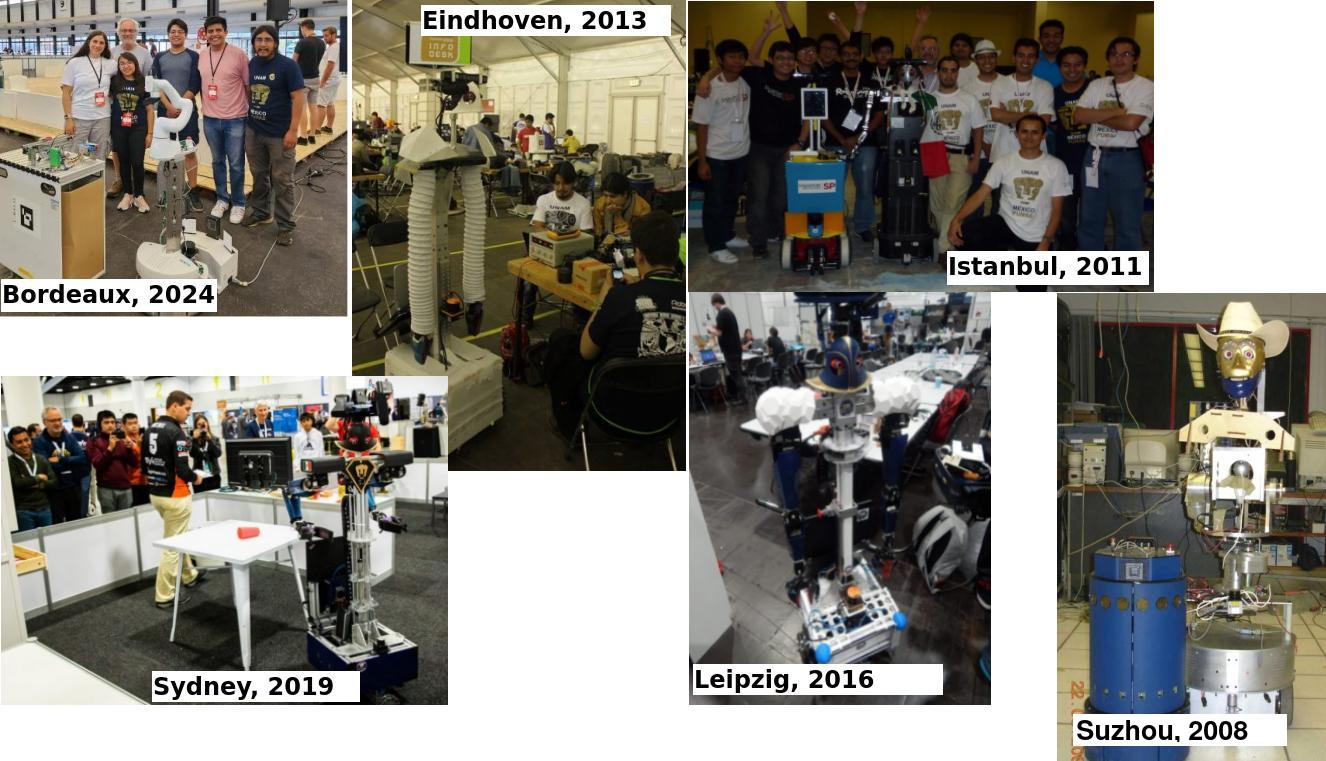
\includegraphics[width=0.9\textwidth]{Figures/Participations.jpg}
\end{frame}

\begin{frame}\frametitle{Nuestro laboratorio}
  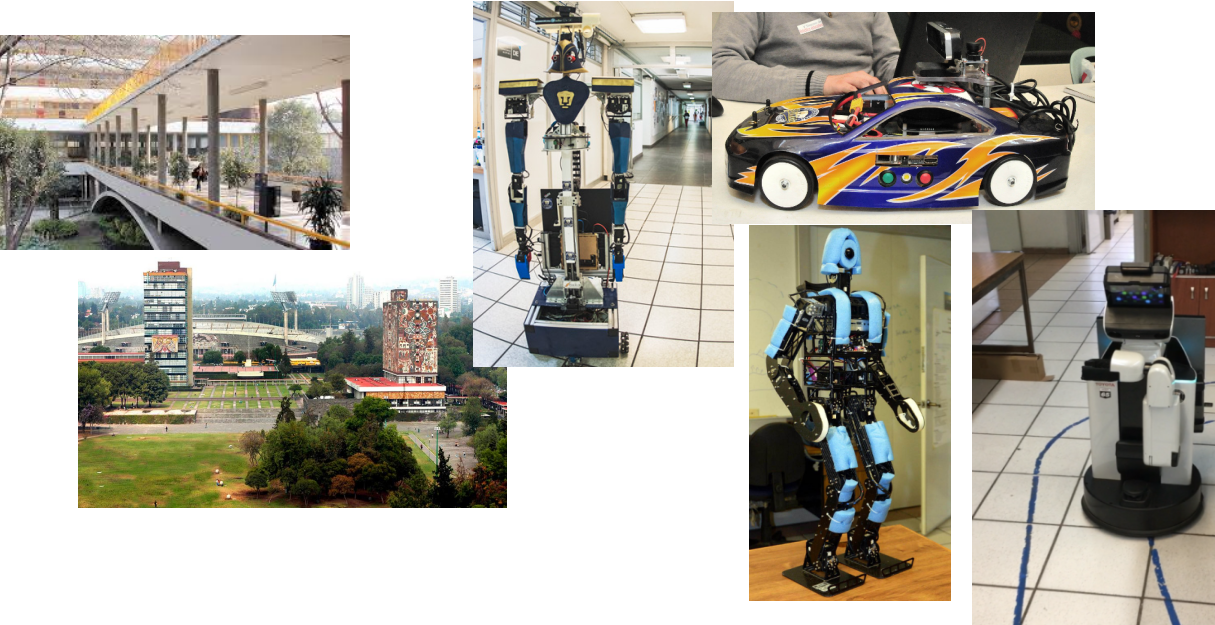
\includegraphics[width=\textwidth]{Figures/Lab.png}
\end{frame}




\section{Introducción}

\begin{frame}\frametitle{Algunos conceptos previos}
    \begin{itemize}
  \item \textbf{Configuración:} es la descripción de la posición en el espacio de todos los puntos del robot. Se denota con $q$.
  \item \textbf{Espacio de configuraciones:} es el conjunto $Q$ de todas las posibles configuraciones. 
  \item \textbf{Grados de libertad:} número mínimo de variables independientes para describir una configuración. En este curso, la base móvil del robot tiene 3 GdL, la cabeza tiene 2 GDL y cada brazo tiene 7 GDL más 1 GdL para el gripper. En total, el robot tiene 21 GdL. 
  \end{itemize}
  \textbf{Propiedades del robot:}
  \begin{itemize}
  \item \textbf{Holonómico:} el robot puede moverse instantáneamente en cualquier dirección del espacion de configuraciones. Comunmente se logra mediante ruedas de tipo \textit{Mecanum} u \textit{Omnidireccionales}. 
  \item \textbf{No holonómico:} existen restricciones de movimiento en velocidad pero no en posición. Son restricciones que solo se pueden expresar en términos de la velocidad pero no pueden integrarse para obtener una restricción en términos de posición. Ejemplo: un coche sólo puede moverse en la dirección que apuntan las llantas delanteras, sin embargo, a través de maniobras puede alcanzar cualquier posición y orientación. El robot de este curso es no holonómico. 
  \end{itemize}
\end{frame}

\begin{frame}\frametitle{Algunos conceptos previos}
  \textbf{Propiedades de los algoritmos:}
  \begin{itemize}
  \item \textbf{Complejidad:} cuánta memoria y cuánto tiempo se requiere para ejecutar un algoritmo, en función del número de datos de entrada (número de grados libertad, número de lecturas de un sensor, entre otros).
  \item \textbf{Optimalidad:} un algoritmo es óptimo cuándo encuentra una solución que minimiza una función de costo.
  \item \textbf{Completitud:} un algoritmo es completo cuando garantiza encontrar la solución siempre que ésta exista. Si la solución no exite, indica falla en tiempo finito.
    \begin{itemize}
    \item Completitud de resolución: la solución existe cuando se tiene una discretización. 
    \item Completitud probabilística: la probabilidad de encontrar la solución tiende a 1.0 cuando el tiempo tiende a infinito.
    \end{itemize}
  \end{itemize}
\end{frame}

\begin{frame}\frametitle{Planeación de movimientos}
El problema de la planeación de movimientos comprende cuatro tareas principales:
  \begin{itemize}
  \item Mapeo: construir una representación del ambiente a partir de las lecuras de los sensores y la trayectoria del robot.
  \item Navegación: encontrar un conjunto de puntos $q \in Q_{free}$ que permitan al robot moverse desde una configuración inicial $q_{start}$ a una configuración final $q_{goal}$.     
  \item Localización: determinar la configuración $q$ dado un mapa y lecturas de los sensores. 
  \item Barrido: pasar un actuador por todos los puntos $q\in Q_b \subset Q$.
  \end{itemize}
\end{frame}

\section{Representación del ambiente}
\begin{frame}\frametitle{Representación del ambiente}
  Un mapa es cualquier representación del ambiente útil en la toma de decisiones.
  \begin{itemize}
  \item Interiores (se suelen representar en 2D)
    \begin{itemize}
    \item Celdas de ocupación
    \item Mapas de líneas
    \item Mapas topológicos: Diagramas de Voronoi generalizados. 
    \item Mapas basados en \textit{Landmarks}
    \end{itemize}
  \item Exteriores (suelen requerir una representación 3D)
    \begin{itemize}
    \item Celdas de elevación
    \item Celdas de ocupación 3D
    \item Octomaps
    \end{itemize}
  \end{itemize}
\end{frame}

\begin{frame}\frametitle{Celdas de ocupación}
  Es un tipo de mapa geométrico. El espacio se discretiza con una resolución determinada y a cada celda se le asigna un número $p\in[0,1]$ que indica su nivel de ocupación. En un enfoque probabilístico este número se puede interpretar como la certeza que se tiene de que una celda esté ocupada.
  \begin{figure}
    \centering
    \includegraphics[width=0.4\textwidth]{Figures/MotionPlanning/OccupancyGrid.png}
    
\includegraphics[width=0.4\textwidth]{Figures/MotionPlanning/OccupancyGridZoom.png}
    \end{figure}
  El mapa resultante se representa en memoria mediante una matriz de valores de ocupación. En ROS, los mapas utilizan el mensaje \texttt{nav\_msgs/OccupancyGrid}.
\end{frame}

\begin{frame}\frametitle{Diagrama de Voronoi Generalizado}
  \begin{itemize}
  \item A diferencia de los mapas geométricos, donde se busca reflejar la forma exacta del ambiente, los \textbf{mapas topológicos} buscan representar solo las relaciones espaciales de los puntos de interés.
  \item Los Diagramas de Voronoi dividen el espacio en regiones. Cada región está asociada a un punto llamado semilla, sitio o generador. Una región asociada a una semilla $x$ contiene todos los puntos $p$ tales que $d(x,p)$ es menor o igual que la distancia $d(x^\prime, p)$ a cualquier otra semilla $x^\prime$.
  \item Un diagrama de Voronoi generalizdo (GVD) considera que las semillas pueden ser objetos con dimensiones y no solo puntos. 
  \end{itemize}
  \begin{figure}
    \centering
    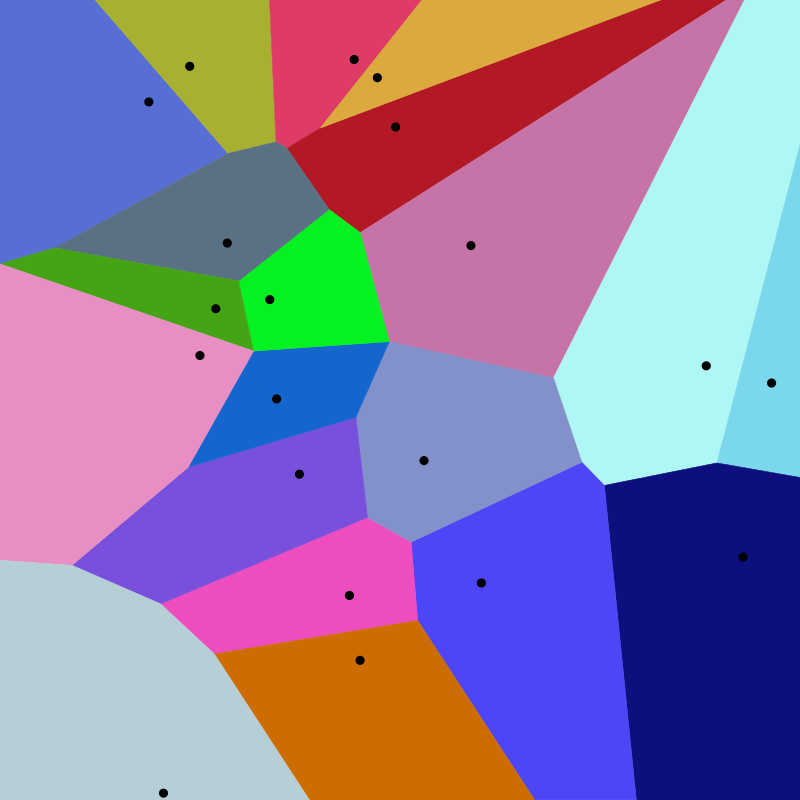
\includegraphics[height=0.4\textheight]{Figures/MotionPlanning/GVD.png}
    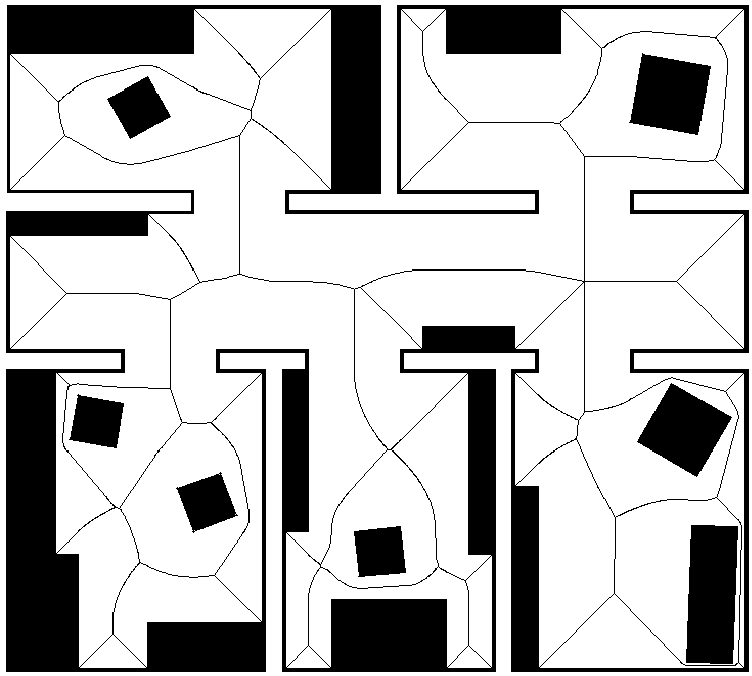
\includegraphics[height=0.4\textheight]{Figures/MotionPlanning/GVDExample.png}
  \end{figure}
  \begin{itemize}
    \item La forma de las regiones depende de la función de distancia que se utilice. 
  \end{itemize}
\end{frame}

\begin{frame}\frametitle{El algoritmo \textit{Brushfire}}
  \begin{columns}
    \begin{column}{0.65\textwidth}
      \begin{itemize}
      \item Obtener un GVD es aún un problema abierto
      \item Se simplifica el problema si se asume un espacio finito y discretizado (celdas de ocupación)
      \item En este caso el GVD se puede obtener mediante el algoritmo \textit{Brushfire}
      \item El mapa de rutas mostrado en la figura se forma con las celdas que son máximos locales en el mapa de distancias devuelto por Brushfire, es decir, son las celdas que son fronteras entre las regiones de Voronoi.
      \item Estas celdas también son aquellas equidistantes a los dos obstáculos más cercanos. 
      \end{itemize}
    \end{column}
    \begin{column}{0.35\textwidth}
      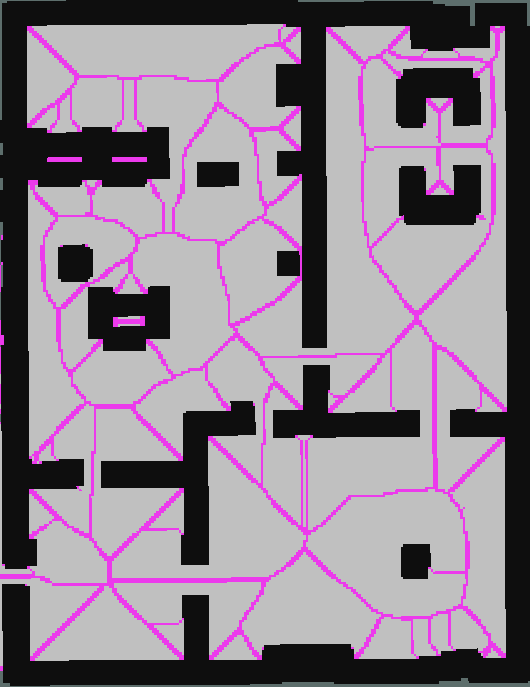
\includegraphics[width=\textwidth]{Figures/MotionPlanning/GVDFromGrid.png}
    \end{column}
  \end{columns}
\end{frame}

\section{Planeación de rutas}
\begin{frame}\frametitle{Planeación de rutas}
  La planeación de rutas consiste en encontrar una secuencia de configuraciones $q\in Q_{free}$ que permitan al robot moverse desde una configuración inicial $q_{start}$ hasta una configuración final $q_{goal}$.
  \begin{itemize}
  \item Una \textbf{ruta} es solo la secuencia de configuraciones para llegar a la meta.
  \item Cuando la secuencia de configuraciones se expresa en función del tiempo, entonces se tiene una \textbf{trayectoria}. 
  \end{itemize}
  En este curso solo vamos a hacer planeación de rutas, no de trayectorias (para navegación).\\
  Existen varios métodos para planear rutas. La mayoría de ellos se pueden agrupar en:
  \begin{itemize}
  \item Métodos basados en muestreo
  \item Métodos basados en grafos
  \end{itemize}
\end{frame}

\begin{frame}\frametitle{Métodos basados muestreo}
  Como su nombre lo indica, consisten en tomar muestras aleatorias del espacio libre. Si es posible llegar en línea recta de la configuración actual al punto muestrado, entonces se agrega a la ruta.
  Ejemplos:
  \begin{itemize}
  \item RRT (Rapidly-exploring Random Trees)
  \item RRT-Bidireccional
  \item RRT-Extendido
  \end{itemize}
\end{frame}

\begin{frame}\frametitle{\textit{Rapidly-exploring Random Trees}}
  Consiste en construir un árbol a partir de muestras aleatorias del espacio libre. Los pasos generales se pueden resumir en:
  \begin{columns}
    \begin{column}{0.55\textwidth}
      \begin{enumerate}
      \item Construir un árbol $T$ con nodo raíz en el punto inicial
      \item Elegir una posición aleatoria $p=(x,y)$ dentro del espacio libre
      \item Encontrar el nodo $n$, del árbol $T$, más cercano al punto $p$
      \item Si la distancia $d(n, p) > \epsilon$, cambiar $p$ por un punto en la misma dirección $\overrightarrow{np}$ pero a una distancia $\epsilon$
      \item Si no hay colisión entre $n$ y $p$, agregar a $p$ como nodo hijo de $n$
      \item Si no hay colisión entre $p$ y el punto meta $p_g$, agregar $p_g$ como nodo hijo de $p$, terminar la exploración y anunciar éxito
      \item Repertir desde el punto 2 un máximo de $N$ veces.
      \end{enumerate}
    \end{column}
    \begin{column}{0.45\textwidth}
      \begin{figure}
        \centering
        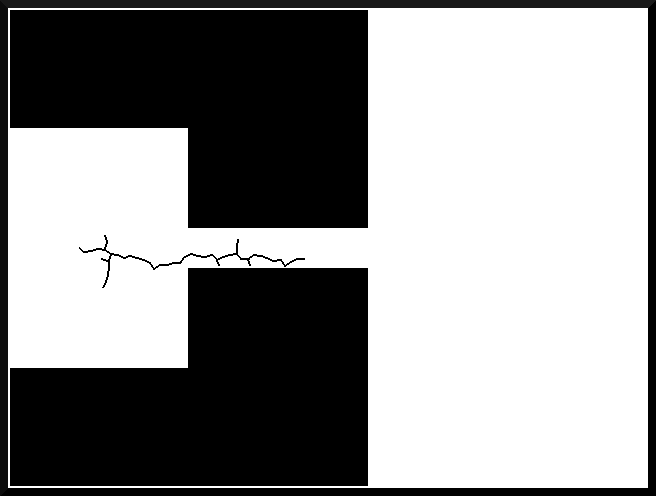
\includegraphics[width=0.45\textwidth]{Figures/MotionPlanning/RRTO010.png}
        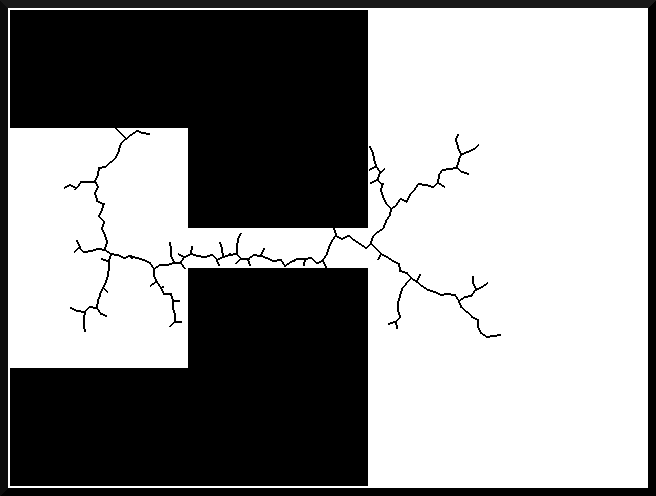
\includegraphics[width=0.45\textwidth]{Figures/MotionPlanning/RRTO0100.png}
        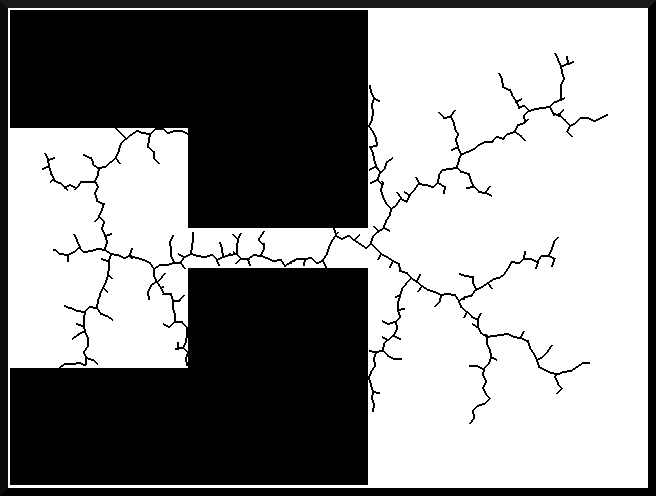
\includegraphics[width=0.45\textwidth]{Figures/MotionPlanning/RRTO0300.png}
      \end{figure}
    \end{column}
  \end{columns}
\end{frame}

\begin{frame}\frametitle{Métodos basados en grafos}
  Estos métodos consideran el ambiente como un grafo. En el caso de celdas de ocupación, cada celda libre es un nodo que está conectado con las celdas vecinas que también estén libres. Los pasos generales de este tipo de algorimos se pueden resumir en:
  \[\]
  \begin{algorithm}[H]
    \footnotesize
    \DontPrintSemicolon
    \KwData {Mapa $M$ de celdas de ocupación, configuración inicial $q_{start}$, configuración meta $q_{goal}$}
    \KwResult{Ruta $P=[q_{start},q_1, q_2, \dots , q_{goal}]$}
    Obtener los nodos $n_s$ y $n_g$ correspondientes a $q_{start}$ y $q_{goal}$\;
    Lista abierta $OL = \emptyset$ y lista cerrada $CL = \emptyset$\;
    Agregar $n_s$ a $OL$\;
    Nodo actual $n_c = n_s$\;
    \While{$OL\neq \emptyset$ y $n_c\neq n_g$}
    {
      Seleccionar $n_c$ de $OL$ \textbf{bajo algún criterio}\;
      Agregar $n_c$ a $CL$\;
      Expandir $n_c$\;
      Agregar a $OL$ los vecinos de $n_c$ que no estén ya en $OL$ ni en $CL$\;
    }
    \If{$n_c\neq n_g$}{Anunciar Falla}
    Obtener la configuración $q_i$ para cada nodo $n_i$ de la ruta\;
  \end{algorithm}
\end{frame}

\begin{frame}\frametitle{Métodos basados en grafos}
  El criterio para seleccionar el siguiente nodo a expandir $n_c$ de la lista abierta, determina el tipo de algoritmo:
  \begin{itemize}
  \item Criterio FIFO: Búsqueda a lo ancho BFS (la lista abierta es una cola)
  \item Criterio LIFO:  Búsqueda en profundidad DFS (la lista abierta es una pila)
  \item Menor valor $g$: Dijkstra (la lista abierta es una cola con prioridad)
  \item Menor valor $f$: A* (la lista abierta es una cola con prioridad)
  \end{itemize}
  Si el costo $g$ para ir de una celda a otra es siempre 1, entonces Dijkstra es equivalente a BFS. \\
  A* y Dijkstra siempre calculan la misma ruta (óptima) pero A* lo hace más rápido. 
\end{frame}

\begin{frame}\frametitle{Inflado de celdas de ocupación}
  Aunque las celdas de ocupación representan el espacio donde hay obstáculos y donde no, en realidad, el robot no puede posicionarse en todas las celdas libres, debido a su tamaño, como se observa en la figura:
  \begin{columns}
    \begin{column}{0.6\textwidth}
      \begin{figure}
        \centering
        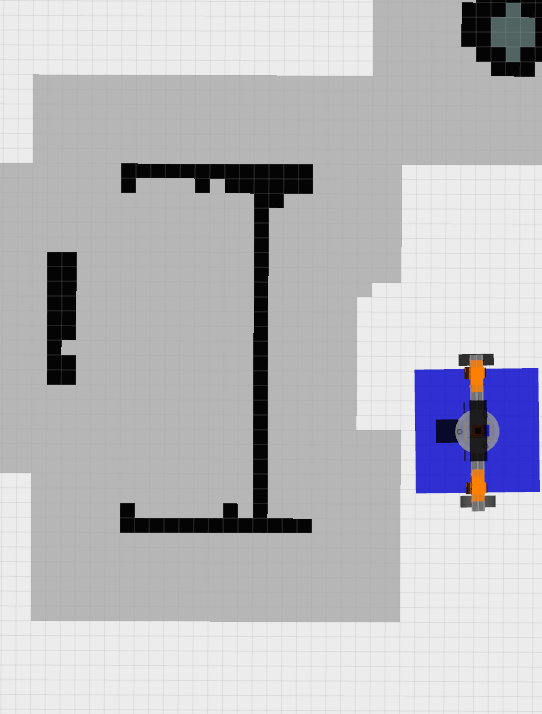
\includegraphics[width=0.45\textwidth]{Figures/MotionPlanning/InflationExample1.png}
        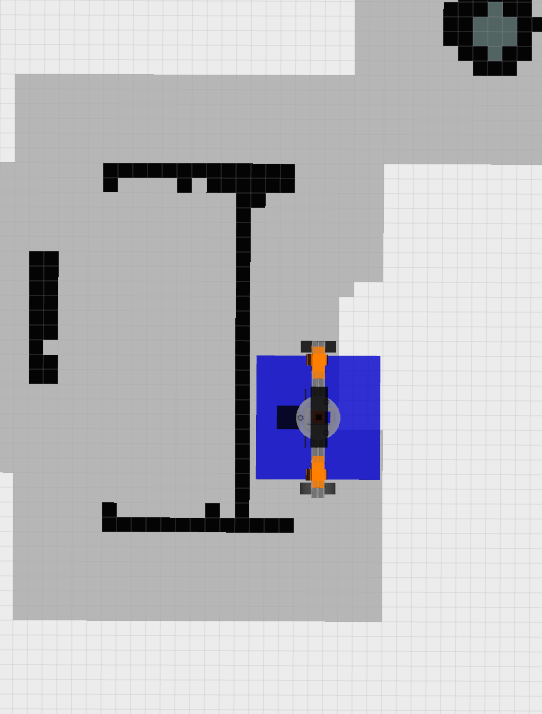
\includegraphics[width=0.45\textwidth]{Figures/MotionPlanning/InflationExample2.png}
      \end{figure}
    \end{column}
    \begin{column}{0.4\textwidth}
      \begin{itemize}
      \item Celdas blancas: espacio libre.
      \item Celdas negras: espacio con obstáculos.
        \item Celdas grises: espacio sin obstáculos donde el robot no puede estar debido a su tamaño. 
      \end{itemize}
    \end{column}
  \end{columns}
  \begin{itemize}
  \item Un mapa de celdas de ocupación debe \textit{inflarse} antes de usarse para planear rutas.
  \item Esta operación se conoce como \textit{dilatación} y es tipo de \textit{operador morfológico}
  \item El inflado se usa para planeación de rutas, no para localización.
  \end{itemize}
\end{frame}

\begin{frame}\frametitle{Mapas de costo}
  \begin{itemize}
  \item Los métodos como Dijkstra y A* minimizan una función de costo. Esta función podría ser distancia, tiempo de recorrido, número de giros, energía gastada, entre otras.
  \item En este curso se empleará como costo una combinación de distancia recorrida más peligro de colisión (cercanía a los obstáculos).
  \item De este modo, las rutas serán un equilibrio entre rutas cortas y rutas seguras.
  \item Ejemplo: la ruta azul es más larga pero más segura. 
  \end{itemize}
  \begin{figure}
    \centering
    \includegraphics[width=0.5\textwidth]{Figures/MotionPlanning/AStarComparison.png}
  \end{figure}
\end{frame}

\begin{frame}\frametitle{Mapas de costo}
  \begin{itemize}
  \item Se utilizará como costo una función de \textit{cercanía}.
  \item Se calcula de forma similar al algoritmo Brushfire, pero la función decrece conforme nos alejamos de los objetos. 
  \end{itemize}
  \begin{columns}
    \begin{column}{0.6\textwidth}
      \begin{algorithm}[H]
        \footnotesize
        \DontPrintSemicolon
        \KwData {\;
          Mapa $M$ de celdas de ocupación\;
          Radio de costo $r_c$
        }
        \KwResult{Mapa de costo $M_c$}
        \;
        $M_c = $ Copia de $M$\;
        \ForEach{$i\in [0,\dots,rows)$}
        {
          \ForEach{$j\in [0,\dots,cols)$}
          {
            //Si está ocupada, calcular el costo de $r_c$ celdas alrededor.\;
            \If{$M[i,j] == 100$ }
            {
              \ForEach{$k_1\in [-r_c,\dots,r_c]$}
              {
                \ForEach{$k_2\in [-r_c,\dots,r_c]$}
                {
                  $C = r_c - max(|k1|,|k2|) + 1$\;
                  $M_c[i+k1,j+k2] = max(C, M_c[i+k1,j+k2]$\;
                }
              }
            }    
          }
        }
        \caption{Mapa de costo}
      \end{algorithm}
    \end{column}
    \begin{column}{0.4\textwidth}
      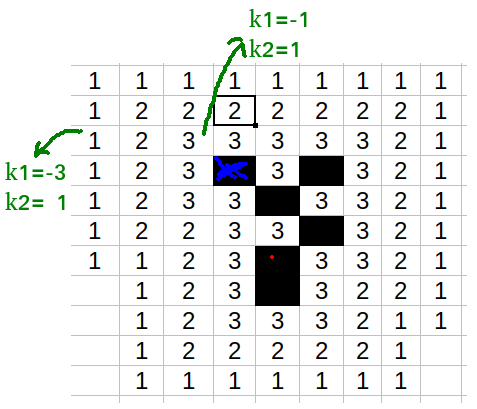
\includegraphics[width=0.95\textwidth]{Figures/MotionPlanning/CostMap.png}
    \end{column}
  \end{columns}
\end{frame}

\begin{frame}\frametitle{El algoritmo A*}
  \begin{itemize}
  \item Es un algoritmo completo, es decir, si la ruta existe, seguro la encontrará, y si no existe, lo indicará en tiempo finito.
  \item Al igual que Dijkstra, A* encuentra una ruta que minimiza una función de costo, es decir, es un algoritmo óptimo.
  \item Es un algoritmo del tipo de búsqueda informada, es decir, utiliza información sobre el estimado del costo restante para llegar a la meta para priorizar la expansión de ciertos nodos. 
  \item El nodo a expandir se selecciona de acuerdo con la función:
    \[f(n) = g(n) + h(n)\]
    donde
    \begin{itemize}
    \item $g(n)$ es el costo acumulado del nodo $n$
    \item $h(n)$ es una función heurística que \textbf{subestima} el costo de llegar del nodo $n$ al nodo meta $n_g$. 
    \end{itemize}
  \item Se tienen los siguientes conjuntos importantes:
    \begin{itemize}
    \item Lista abierta: conjunto de todos los nodos en la frontera (visitados pero no conocidos). Es una cola con prioridad donde los elementos son los nodos y la prioridad es el valor $f(n)$.
    \item Lista cerrada: conjunto de nodos para los cuales se ha calculado una ruta óptima. 
    \end{itemize}
    \item A cada nodo se asocia un valor $g(n)$, un valor $f(n)$ y un nodo padre $p(n)$. 
  \end{itemize}
\end{frame}

\begin{frame}\frametitle{El algoritmo A*}
    \begin{algorithm}[H]
    \footnotesize
    \DontPrintSemicolon
    \KwData {Mapa $M$, nodo inicial $n_s$ con configuración $q_{s}$, nodo meta $n_g$ con configuración $q_{g}$}
    \KwResult{Ruta óptima $P=[q_{s},q_1, q_2, \dots , q_{g}]$}
    Lista abierta $OL = \emptyset$ y lista cerrada $CL = \emptyset$\;
    Fijar $f(n_{s}) = 0$, $g(n_{s}) = 0$ y $prev(n_{s}) = NULL$\;
    Agregar $n_s$ a $OL$ y fijar nodo actual $n_c = n_s$\;
    \While{$OL\neq \emptyset$ y $n_c\neq n_g$}
    {
      Remover de $OL$ el nodo $n_c$ con el menor valor $f$ y agregar $n_c$ a $CL$\;
      \ForAll{$n$ vecino de $n_c$}
      {
        $g = g(n_c) + costo(n_c, n)$\;
        \If{$g < g(n)$}
        {
          $g(n) = g$\;
          $f(n) = h(n) + g(n)$\;
          $prev(n) = n_c$\;
        }
      }
      Agregar a $OL$ los vecinos de $n_c$ que no estén ya en $OL$ ni en $CL$\;
    }
    \If{$n_c\neq n_g$}{Anunciar Falla}
    \While{$n_c \neq NULL$}
    {
      Insertar al inicio de la ruta $P$ la configuración correspondiente al nodo $n_c$\;
      $n_c = prev(n_c)$
    }
    Devolver ruta óptima $P$
  \end{algorithm}
\end{frame}

\begin{frame}\frametitle{El algoritmo A*}
  \begin{itemize}
  \item La función de costo será el número de celdas más el mapa de costo obtenido anteriormente.
  \item Puesto que el mapa está compuesto por celdas de ocupación, los nodos vecinos se pueden obtener usando conectividad 4 o conectividad 8.
  \item Si se utiliza conectividad 4, la distancia de Manhattan es una buena heurística.
  \item Si se utiliza conectividad 8, se debe usar la distancia Euclideana.
  \item La lista abierta se puede implementar con una \textit{Heap}, de este modo, la inserción de los nodos $n$ se puede hacer en tiempo logarítmico y la selección del nodo con menor $f$ se hace en tiempo constante.
  \end{itemize}
\end{frame}

\section{Seguimiento de rutas}
\begin{frame}\frametitle{Seguimiento de rutas}
  Hasta el momento ya se tiene una representación del ambiente y una forma de planear rutas. Ahora falta diseñar las leyes de control que hagan que el robot se mueva por la ruta calculada. Este control se hará bajo los siguientes supuestos:
  \begin{itemize}
  \item Se conoce la posición del robot (más adelante se abodará el problema de la localización)
  \item El modelo cinemático es suficiente para modelar el movimiento del robot 
  \item Las dinámicas no modeladas (parte eléctrica y mecánica de los motores) son lo suficientemente rápidas para poder despreciarse
  \end{itemize}
\end{frame}

\begin{frame}\frametitle{Base diferencial}
  \begin{itemize}
  \item Es la configuración más sencilla debido a la simplicidad del hardware requerido
  \item Aunque implica restricciones no holonómicas, es suficiente para la mayoría de los movimientos requeridos. Además, suponer este tipo de base es algo útil debido a una razón sencilla: los sensores suelen estar al frente del robot. 
  \item Se diseñarán leyes de control suponiendo esta configuración.
  \end{itemize}
  \begin{columns}
    \begin{column}{0.4\textwidth}
      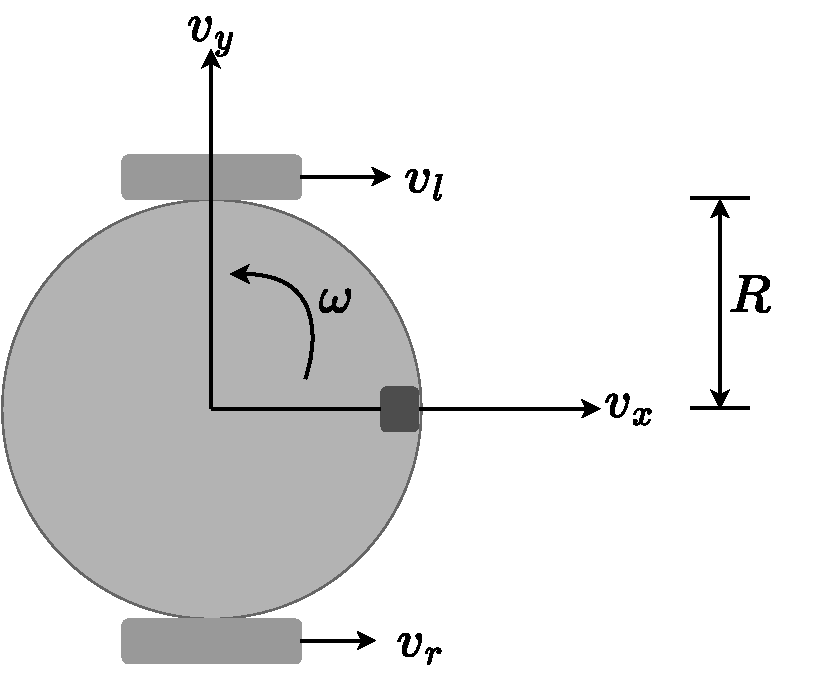
\includegraphics[width=\textwidth]{Figures/MotionPlanning/DifferentialBase.pdf}
    \end{column}
    \begin{column}{0.6\textwidth}
      \begin{eqnarray*}
        v_l &=& v_x - R\omega\\
        v_r &=& v_x + R\omega
      \end{eqnarray*}
    \end{column}
  \end{columns}
\end{frame}

\begin{frame}\frametitle{Control de posición}
  \begin{columns}
    \begin{column}{0.5\textwidth}
      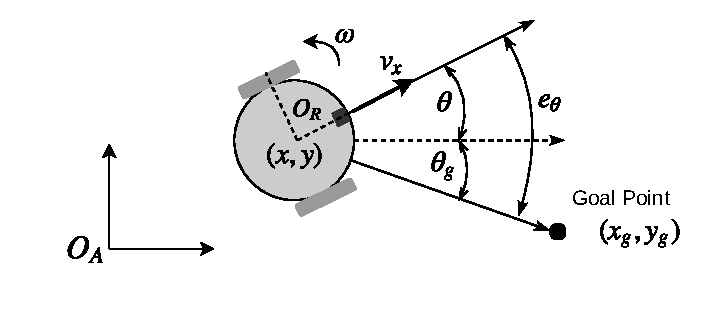
\includegraphics[width=0.95\textwidth]{Figures/MotionPlanning/GoalPose.pdf}
    \end{column}
    \begin{column}{0.5\textwidth}
      Considere una base diferencial y el punto meta $(x_g, y_g)$, las siguientes leyes de control permiten al robot alcanzar dicho punto meta:
      \begin{eqnarray*}
        v_x    &=& v_{max}e^{-\frac{e_{\theta}^{2}}{\alpha}}\label{eq:Control11}\\
        \omega &=& \omega_{max}\left(\frac{2}{1+e^{-\frac{e_{\theta}}{\beta}}}-1\right)\label{eq:Control12}
      \end{eqnarray*}
    \end{column}
  \end{columns}
  con
  \[e_{\theta} = \atantwo\left(y_g - y, x_g - x\right) - \theta\]
  El error de ángulo $e_\theta$ debe estar siempre en $(-\pi, \pi]$. Esto se puede asegurar con:
  \[e_\theta \leftarrow \left(e_\theta + \pi\right)\% (2\pi) - \pi\]
  donde \% denota el operador módulo. 
\end{frame}

\begin{frame}\frametitle{Control de posición}
  \begin{itemize}
  \item $v_{max}$ y $\omega_{max}$ son las velocides lineal y angular máximas.
  \item $\alpha$ y $\beta$ determinan qué tan rápido cambian las velocidades cuando cambia el error de posición.
  \item En general, valores pequeños de $\alpha$ y $\beta$ hacen que el robot siga la ruta más de cerca pero valores muy pequeños pueden producir \textit{chattering}.
    \item Valores grandes de  $\alpha$ y $\beta$ producen un movimiento más suave pero puede resultar en curvas muy extendidas. 
  \end{itemize}
  \begin{figure}
    \centering
    \includegraphics[width=0.45\textwidth]{Figures/MotionPlanning/LinearSpeed.eps}
    \includegraphics[width=0.45\textwidth]{Figures/MotionPlanning/AngularSpeed.eps}
  \end{figure}
\end{frame}


\begin{frame}\frametitle{Perfil de velocidad}
  \begin{columns}
    \begin{column}{0.43\textwidth}
      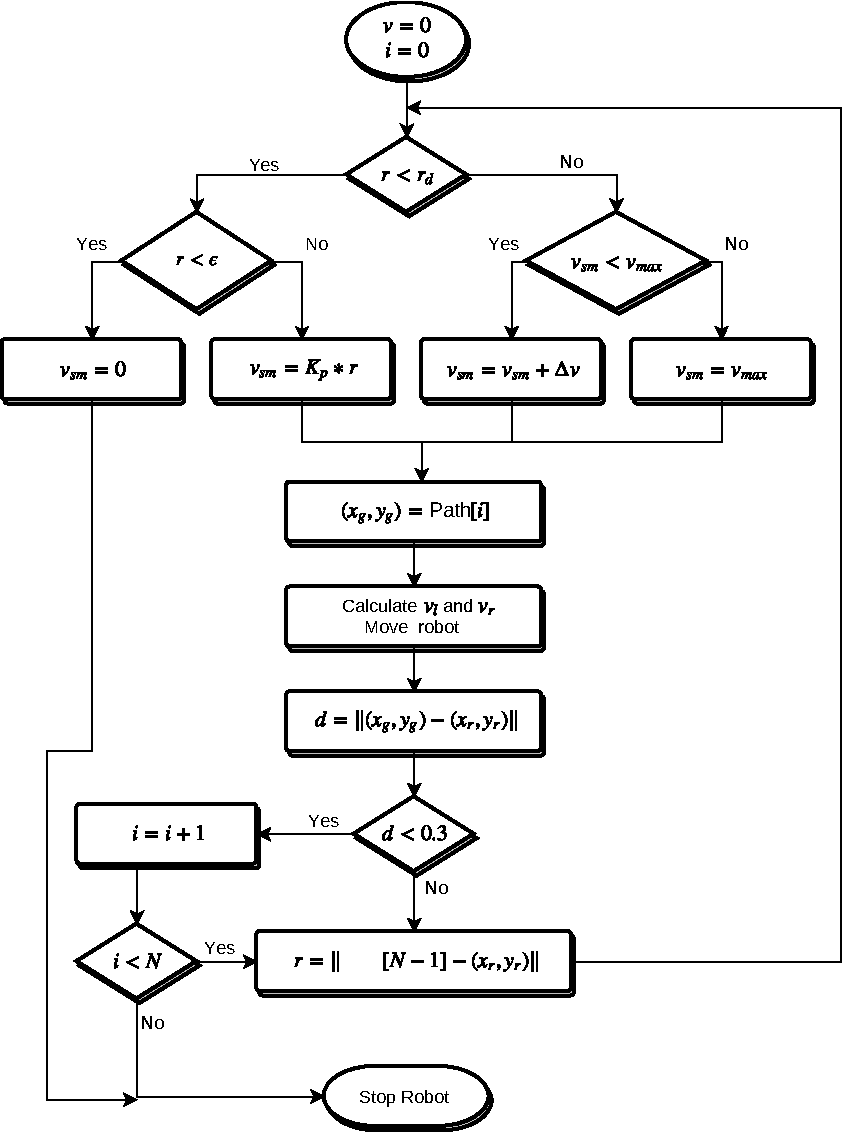
\includegraphics[width=\textwidth]{Figures/MotionPlanning/AFSM.pdf}
    \end{column}
    \begin{column}{0.5\textwidth}
      Considere una máquina de estados finita para calcular $v_{max}$. Sea $v_{sm}$ la nueva velocidad lineal máxima, tal que, ahora el control está dado por:
      \begin{eqnarray*}
        v      &=& v_{sm}e^{-\frac{e_{\theta}^{2}}{\alpha}}\label{eq:NewControl1}\\
        \omega &=& \omega_{max}\left(\frac{2}{1+e^{-\frac{e_{\theta}}{\beta}}}-1\right)\label{eq:NewControl2}
      \end{eqnarray*}
      con
      \begin{itemize}
      \item $r$: Distancia la punto meta
      \item $\epsilon$: Tolerancia para considerar que se alcanzó el punto meta
      \item $r_d$: Distancia al punto meta para empezar a desacelerar
      \item $\Delta v$: Aceleración deseada
      \end{itemize}
    \end{column}
  \end{columns}
\end{frame}

\begin{frame}\frametitle{Perfil de velocidad}
  La figura muestra un ejemplo de una ruta planeada y el perfil de velocidad generada usando solo las leyes de control y usando la AFSM para generar un perfil de velocidad. 
  \begin{figure}
    \centering
    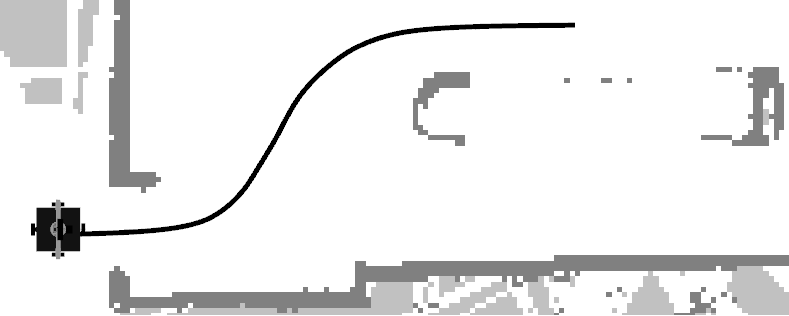
\includegraphics[width=0.45\textwidth]{Figures/MotionPlanning/SpeedProfilePath.png}
  \end{figure}
  \begin{figure}
    \centering
    \includegraphics[width=0.45\textwidth]{Figures/MotionPlanning/SpeedWithoutProfile.eps}
    \includegraphics[width=0.45\textwidth]{Figures/MotionPlanning/SpeedWithProfile.eps}
  \end{figure}
\end{frame}

% \section{Path smoothing}
\begin{frame}\frametitle{Suavizado de rutas}
  \begin{itemize}
  \item Puesto que las rutas se calcularon a partir de celdas de ocupación, están compuestas de esquinas.
  \item La esquinas no son deseables, pues suelen generar cambios bruscos en las señales de control.
  \item La ruta verde de la imagen es una muestra de una ruta calculada por A*.
  \item Es preferible una ruta como la azul. 
  \end{itemize}
  \begin{figure}
    \centering
    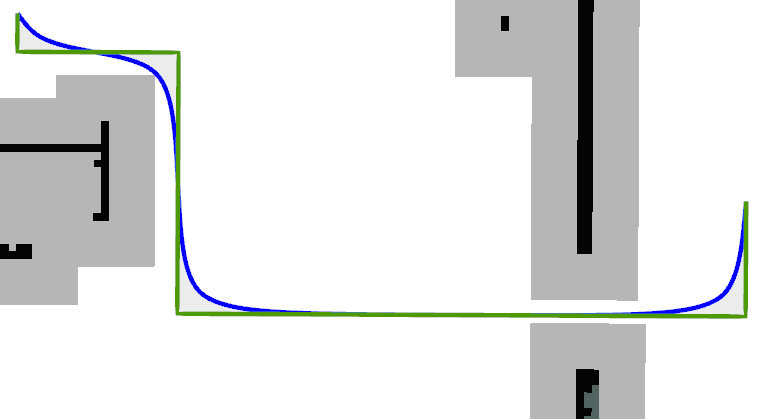
\includegraphics[height=0.45\textheight]{Figures/MotionPlanning/PathSmoothingExample.png}
  \end{figure}
  Usaremos un enfoque de optimización para suavizar la ruta generada por A*
\end{frame}

\begin{frame}\frametitle{Suavizado mediante descenso del gradiente}
  Se plantea una función de costo tal que, minimizar dicha función, resulte en una ruta suavizada. Los puntos negros representan la ruta de A* compuesta por los puntos $Q=\{q_0, q_1, \dots, q_n\}$ y los puntos azules representan una ruta suave $P=\{p_0, p_1,\dots, p_n\}$.
  \begin{columns}
    \begin{column}{0.5\textwidth}
      \begin{figure}
        \centering
        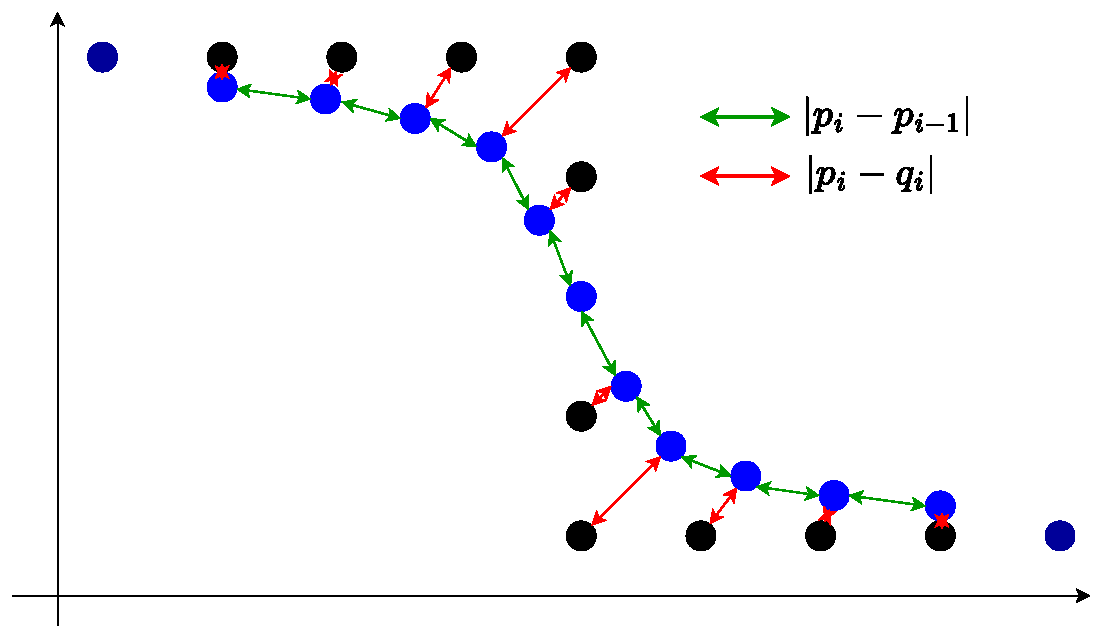
\includegraphics[width=\textwidth]{Figures/MotionPlanning/PathSmoothing.pdf}
      \end{figure}
    \end{column}
    \begin{column}{0.5\textwidth}
      Considere la función de costo:
      \[J = \alpha\frac{1}{2}\sum_{i=1}^{n-1}\left(p_i - p_{i-1}\right)^2 + \beta\frac{1}{2}\sum_{i=1}^{n-1}(p_i - q_i)^2\]
      \begin{itemize}
      \item $J$ es la suma de distancias entre un punto y otro de la ruta suavizada, y entre la ruta suavizada y la original.
      \item Si la ruta es muy suave, $J$ es grande.
      \item Si la ruta es muy parecida a la original, $J$ también es grande.
      \item Una ruta ni muy suave ni muy parecida a la original, logrará minimizar $J$.
      \end{itemize}
    \end{column}
  \end{columns}
\end{frame}

\begin{frame}\frametitle{Suavizado mediante descenso del gradiente}
  \begin{itemize}
  \item Una forma de encontrar el mínimo es resolviendo $\nabla J(p) = 0$, y luego evaluando la matriz Hessiana para determinar si el punto crítico $p_c$ es un mínimo.
  \item Esto se puede complicar debido al alto número de variables en $p$.
  \item Una forma más sencilla, es mediante el descenso del gradiente.
  \end{itemize}
  \begin{columns}
    \begin{column}{0.7\textwidth}
  \begin{algorithm}[H]
    \footnotesize
  \DontPrintSemicolon
  \KwData {Función $J(p):\mathbb{R}^n\rightarrow \mathbb{R}$ a minimizar}
  \KwResult{Vector $p$ que minimiza la función $J$}
  $p\leftarrow p_{init}$ //Fijar una estimación inicial\;
  \While{$|\nabla J(p)| > tol$}
  {
    $p \leftarrow p - \epsilon \nabla J (p)$ //$p$ se modifica un poco en sentido contrario al gradiente.\;
  }
  Devolver $p$
  \caption{Descenso del gradiente}
\end{algorithm}
\end{column}
\end{columns}
\[\]
El descenso del gradiente devuelve el mínimo local más cercano a la condición inicial $p_0$. Pero la función de costo $J$ tiene solo un mínimo global. El gradiente de la función de costo $J$ se calcula como:
  \[\underbrace{\left[\frac{}{}\alpha(p_0 - p_1)+\beta(p_0 - q_0)\right. }_{\dfrac{\partial J}{\partial p_0}}
,\dots ,
\underbrace{\frac{}{}\alpha(2p_i - p_{i-1} - p_{i+1})+\beta(p_i - q_i)}_{\dfrac{\partial J}{\partial p_i}}
,\dots ,
\underbrace{\left.\alpha(p_{n-1} - p_{n-2})+\beta(p_{n-1}-q_{n-1})\frac{}{}\right]}_{\dfrac{\partial J}{\partial p_{n-1}}}
\]
\end{frame}

\begin{frame}\frametitle{Suavizado mediante descenso del gradiente}
  
  Para no variar los puntos inicial y final de la ruta, la primer y última componentes de $\nabla J$ se dejarán en cero. El algoritmo de descenso del gradiente queda como:
  \[\]
\begin{algorithm}[H]
\DontPrintSemicolon
  \DontPrintSemicolon
  \KwData{Conjunto de puntos $Q = \{q_0\dots q_i \dots q_{n-1}\}$ de la ruta original, parámetros $\alpha$ y $\beta$, ganancia $\epsilon$ y tolerancia $tol$\;}
  \KwResult{Conjunto de puntos $P = \{p_0\dots p_i \dots p_{n-1}\}$ de la ruta suavizada\;}
  $P \leftarrow Q$\;
  $\nabla J_0 \leftarrow 0$\;
  $\nabla J_{n-1} \leftarrow 0$\;   
  \While{ $\Vert\nabla J(p_i)\Vert > tol \wedge$ steps < max\_steps}
  {
    \ForEach{$i \in [1,n-1)$}
    {
      $\nabla J_i \leftarrow \alpha (2p_i - p_{i-1} - p_{i+1}) + \beta (p_i - q_i)$\;
    }
    $P \leftarrow P - \epsilon \nabla J$\;
    $steps \leftarrow steps + 1$
  }
  regresar $P$
  \caption{Suavizado de rutas mediante descenso del gradiente}
\end{algorithm}
\end{frame}

\section{Localización}
\section{Localización (2024-09-05)}
\begin{frame}\frametitle{Localización}
  El problema de la localización consiste en determinar la configuración $q$ del robot dada un mapa y un conjunto de lecturas de los sensores.
  \begin{itemize}
  \item La localización se podría lograr simplemente integrando los comandos de velocidad del robot.
  \item Si se conoce perfectamente la configuración inicial y el robot ejecuta perfectamente los comandos de movimiento, entonces la simple integración de la velocidad de los motores sería suficiente.
  \item Esto por supuesto no es posible. Se tiene incertidumbre tanto en la estimación inicial de la posición como en la ejecución de cada movimiento.
  \item Es decir, el robot pierde información sobre su posición en cada movimiento. 
  \end{itemize}
\end{frame}

\begin{frame}\frametitle{Localización}
  Existen principalmente dos tipos:
\[\]
  \begin{columns}
    \begin{column}{0.5\textwidth}
      \textbf{Localización local: }
      \begin{itemize}
      \item Requiere una estimación inicial \textit{cercana} a la posición real del robot, de otro modo, no converge.
      \item Suele ser menos costosa computacionalmente.
      \item Un método común es el Filtro de Kalman Extendido.
      \end{itemize}
    \end{column}
    \begin{column}{0.5\textwidth}
      \textbf{Localización global:}
      \begin{itemize}
      \item La estimación inicial puede ser cualquiera.
      \item Suele ser computacionalmente costosa.
      \item Un método común son los Filtros de Partículas. 
      \end{itemize}
      \[\]
      \[\]
    \end{column}
  \end{columns}
\end{frame}

\begin{frame}\frametitle{Localización probabilística}
  \begin{itemize}
  \item En la localización probabilística, en lugar de llevar una sola estimación sobre la posición del robot, se mantiene una \textit{distribución de probabilidad} sobre todo el espacio de hipótesis.
  \item El enfoque probabilístico permite manejar las incertidumbres inherentes al movimiento y al sensado.
  \item El reto es obtener una distribución de densidad de probabilidad (PDF) sobre todas las posibles posiciones del robot.
  \item En general, los métodos probabilísticos de estimación se componen de dos pasos:
    \begin{enumerate}
    \item \textbf{Predicción:} Se modifica la PDF de la posición del robot con base en los comandos y el modelo de movimiento.
    \item \textbf{Actualización:} Se corrige la predicción mezclando la información de PDF predicha con información de los sensores. Se obtiene una PDF de la posición y se repite el proceso. 
    \end{enumerate}
  \end{itemize}  
\end{frame}

\begin{frame}\frametitle{El Filtro de Kalman Extendido}
  \begin{itemize}
  \item Es un tipo de filtro Bayesiano que supone que la distribución de probabilidad de la posición del robot es una distribución normal:
    \[x_{k+1} = f(x_k, u_k) + n_p\]
    con:
    \begin{itemize}
    \item $x_{k+1} = f(x_k, u_k)$ : modelo de movimiento del robot (indica la media de la posición, que se distribuye normalmente)
    \item $n_p$ : ruido de proceso, que se distribuye normalmente con media cero y covarianza conocida $Q$
    \end{itemize}
  \item Supone que las mediciones son varibles aleatorias también con una distribución normal
    \[y_{k} = h(x_k) + n_m\]
    con:
    \begin{itemize}
    \item $y_{k} = h(x_k)$ : medición esperada en función de la posición del robot
    \item $n_p$ : ruido de medición, que se distribuye normalmente con media cero y covarianza conocida $R$
    \end{itemize}
  \item Si el sistema es lineal, el Filtro de Kalman converge para cualquier condición inicial
  \item Si el sistema es no lineal (el caso del robot), el Filtro de Kalman converge solo si la estimación inicial es \textit{cercana} a la posición inicial real.
  \item El Filtro de Kalman es un método de localización local
  \end{itemize}
\end{frame}

\begin{frame}\frametitle{El Filtro de Kalman Extendido}
  \begin{itemize}
  \item El EKF pondera dos fuentes de información:
    \[x_{k+1} = f(x_k, u_k) + n_p\]
    \[y_{k} = h(x_k) + n_m\]
    \begin{itemize}
    \item La posición que predice el modelo de movimiento
    \item La posición que mide el sensor
    \end{itemize}
  \item Cada fuente de información tiene una incertidumbre caracterizada por las covarianzas $Q$ y $R$
  \item El EKF pondera ambas fuentes dándole más peso a la fuente con menos incertidumbre
  \end{itemize}
\end{frame}

\begin{frame}\frametitle{El Filtro de Kalman Extendido}
  \begin{figure}
    \centering
    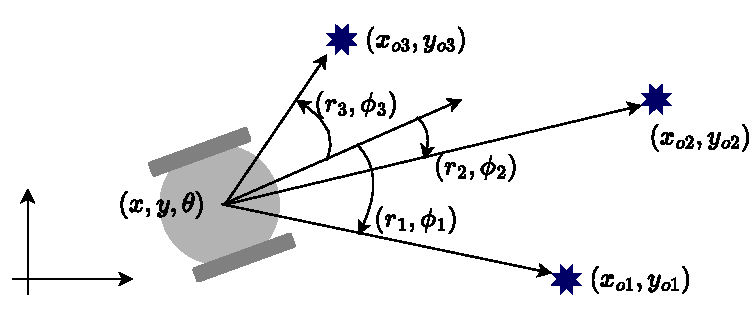
\includegraphics[height=0.4\textheight]{Figures/MotionPlanning/EKF1.pdf}
  \end{figure}
  \begin{columns}
    \begin{column}{0.45\textwidth}
      Modelo de transición de estados:
      \[\left.
      \begin{array}{cclc}
        x_{k+1}      &=& x_k + (\Delta t)v\cos(\theta_k) & + n_{p1}\\
        y_{k+1}      &=& y_k + (\Delta t)v\sin(\theta_k) & + n_{p2}\\
        \theta_{k+1} &=& \theta_k + (\Delta t)\omega     & + n_{p3}
      \end{array}\right\}f(x)
    \]
    donde $n_p\in\mathbb{R}^3$ es ruido de proceso que es distribuye normalmente con
    media cero y matriz de covarianza conocida $Q\in\mathbb{R}^{3\times 3}$
    \end{column}
    \begin{column}{0.55\textwidth}
      Modelo de observación:
      \[\left.
        \begin{array}{cclc}
                 &\vdots& & \\
        r_{i}    &=& \sqrt{(x_k - x_{oi})^2 + (y_k - y_{oi})^2}   & + n_{m1}\\
        \phi_{i} &=& atan2(y_k - y_{oi}, x_k - x_{oi}) - \theta_k & + n_{m2}\\
                 &\vdots& & \\
      \end{array}\right\}h(x)
    \]
    donde $M$ es el número de marcas observadas, $n_m\in\mathbb{R}^{2M}$ es ruido de medición que se distribuye normalmente con media cero y matriz de covarianza conocida $R\in\mathbb{R}^{2M\times 2M}$
    \end{column}
  \end{columns}
\end{frame}

\begin{frame}\frametitle{Algoritmo de estimación del EKF}
  \begin{figure}
    \centering
    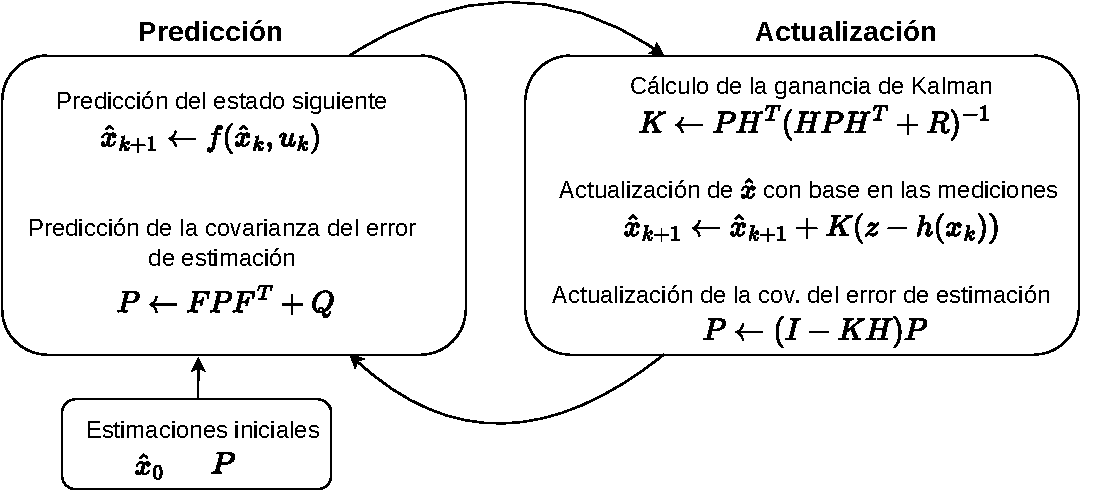
\includegraphics[height=0.6\textheight]{Figures/MotionPlanning/EKFAlgorithm.pdf}
  \end{figure}
  con:
  \begin{itemize}
  \item $P$ : Matriz de covarianza del error de estimación
  \item $F$ : Jacobiano de $f(x)$
  \item $H$ : Jacobiano de $h(x)$
  \item $z$ : Mediciones de los sensores
  \end{itemize}
\end{frame}

\begin{frame}\frametitle{Filtros de partículas}
  \begin{itemize}
  \item También son un filtro Bayesiano
  \item A diferencia del EKF que supone una distribución normal, los filtros de partículas suponen una distribución no paramétrica.
  \item Se consideran $N$ suposiciones de la posición del robot. A cada suposición $(x,y,\theta)$ se le llama partícula. 
  \item La distribución \textit{a priori} se calcula realizando simulaciones de movimiento para cada partícula.
  \item El modelo de observación también se realiza mediante simulaciones de los sensores para cada partículas.
  \item Para obtener la distribución \textit{a posteriori} se comparan las lecturas simuladas con la lectura del sensor real y se realiza un muestreo aleatorio con reemplazo. Cada partícula tiene una probabilidad de ser muestreada, proporcional a la similitud de su lectura simulada con el sensor real.
  \end{itemize}
\end{frame}

\begin{frame}\frametitle{Filtros de Partículas}
  Un filtro de partículas para localización consta de 5 pasos generales:
  \begin{enumerate}
  \item Generar $N$ partículas con $(x,y,\theta)$ aleatorias con distribución uniforme (distribución inicial equivalente a $\hat{x}_0$ en el EKF)
  \item Mover cada partícula un desplazamiento $(\Delta x, \Delta y, \Delta\theta)$ más ruido Gaussiano (equivalente a estimar $\hat{x}_{k+1} = f(x_k, u_k)$ en el EKF)
  \item Simular las lecturas del sensor láser para cada partícula (equivalente a predecir las salidas $h(x_k)$ en el EKF)
  \item Comparar cada lectura simulada con la lectura del sensor real. Las similitudes representan una distribución de probabilidad 
  \item Remuestrear $N$ partículas con reemplazo usando la distribución anterior, y agregar ruido Gaussiano (equivalente a la actualización de la estimación de $\hat{x}$ en el EKF)
  \end{enumerate}
\end{frame}

\begin{frame}\frametitle{Filtros de Partículas}
  \begin{figure}
    \centering
    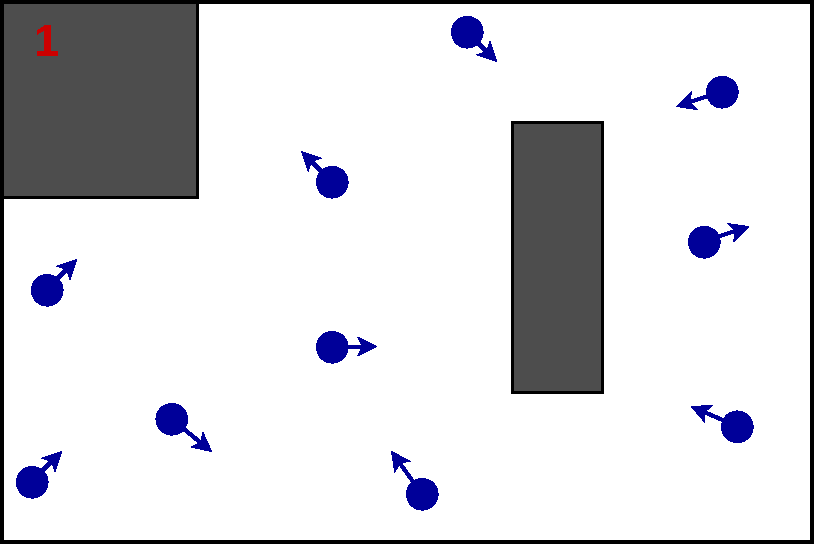
\includegraphics[width=0.30\textwidth]{Figures/MotionPlanning/ParticleFilter1.pdf}
    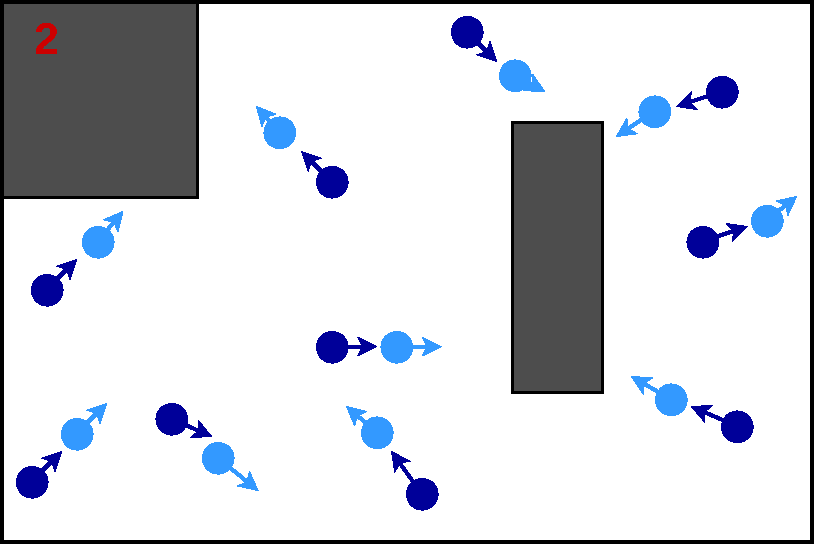
\includegraphics[width=0.30\textwidth]{Figures/MotionPlanning/ParticleFilter2.pdf}
    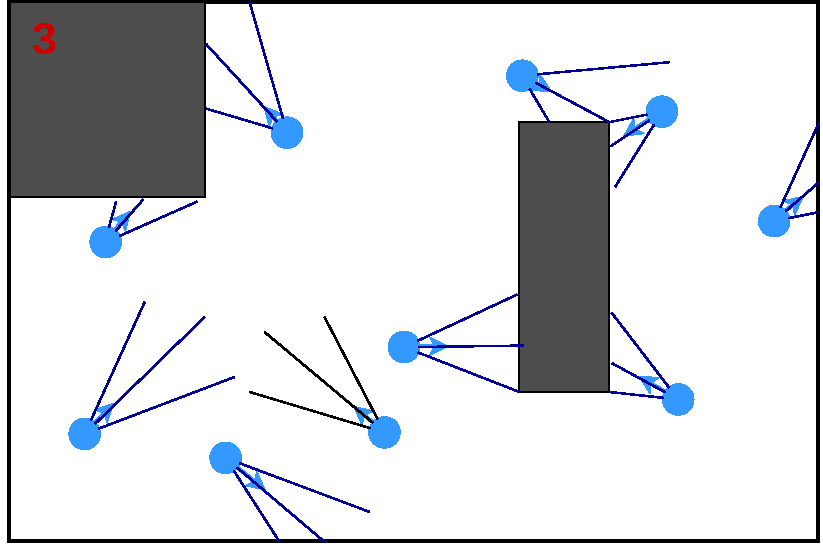
\includegraphics[width=0.30\textwidth]{Figures/MotionPlanning/ParticleFilter3.pdf}
    \includegraphics[width=0.31\textwidth]{Figures/MotionPlanning/ParticleFilter4.pdf}
    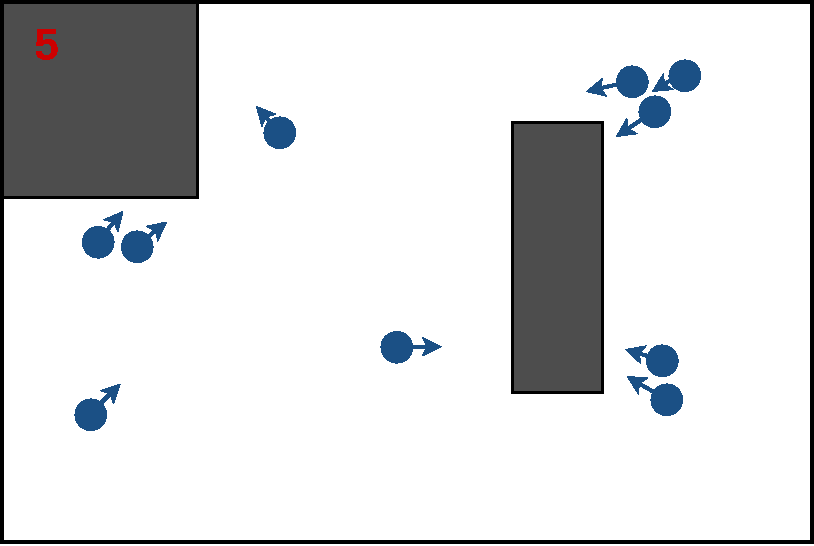
\includegraphics[width=0.30\textwidth]{Figures/MotionPlanning/ParticleFilter5.pdf}
  \end{figure}
\end{frame}

\begin{frame}\frametitle{Desplazamiento de partículas}
  \begin{figure}
    \centering
    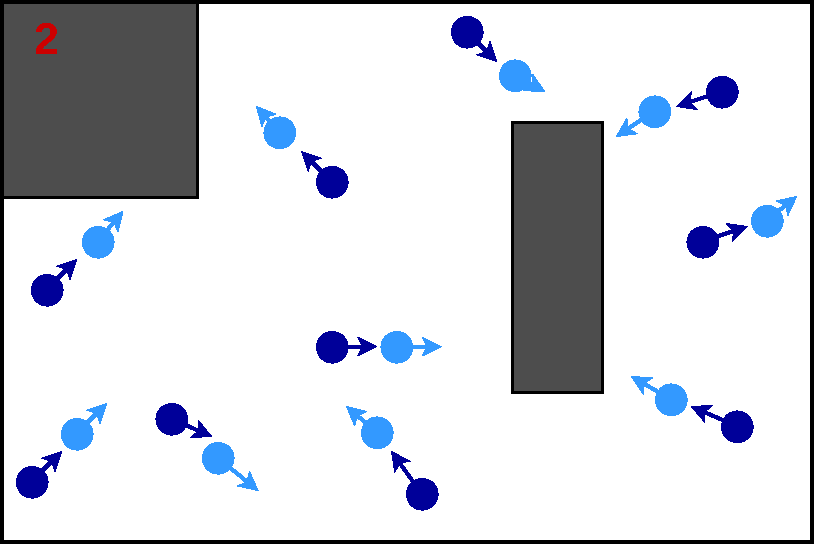
\includegraphics[width=0.35\textwidth]{Figures/MotionPlanning/ParticleFilter2.pdf}
  \end{figure}
  \begin{itemize}
  \item Se puede suponer que todas las partículas se desplazan una cantidad $(\Delta x, \Delta y, \Delta\theta)$ (obtenida mediante odometría) con respecto al sistema del robot
  \item Para calcular la nueva pose de cada partícula, basta con transformar los desplazamientos al sistema de referencia (giro sobre $Z$ de un ángulo $\theta$)
  \item Para modelar la incertidumbre del movimiento, a cada partícula se le suma ruido Gaussiano $n$ con media cero y varianza $\sigma_m^2$:
  \end{itemize}
  Para cada partícula, hacer:
  \begin{eqnarray*}
    x_{k+1} &=& x_k + \Delta x\cos\theta_k - \Delta y\sin\theta_k + n_x\\
    y_{k+1} &=& y_k + \Delta x\sin\theta_k + \Delta y\cos\theta_k + n_y\\
    \theta_{k+1} &=& \theta_k  + \Delta\theta + n_{\theta}
  \end{eqnarray*}
\end{frame}

\begin{frame}\frametitle{Simulación del sensor}
  \begin{itemize}
  \item Se puede simular con técnicas de \textit{ray tracing} a partir de un mapa y una pose del sensor
  \item Se puede utilizar el paquete \texttt{occupancy\_grid\_utils}. Tiene una biblioteca que simula las lecturas del láser dado:
    \begin{itemize}
    \item Un mapa de celdas de ocupación (\texttt{OccupancyGrid})
    \item Una posición y orientación del sensor (\texttt{Pose}). Esta posición y orientación corresponde con el $(x,y,\theta)$ de cada partícula.
    \item Especificaciones del sensor a simular. Esto lo obtiene de un mensaje \texttt{LaserScan}
    \end{itemize}
  \item Puesto que esta simulación es computacionalmente costosa, solo se simulan \textbf{1 de cada $N$} lecturas del sensor real. 
  \end{itemize}
  \begin{figure}
    \centering
    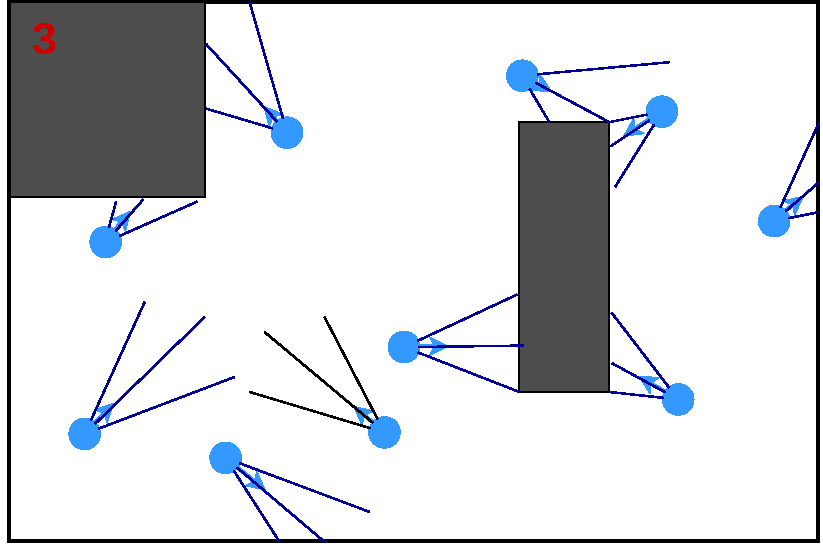
\includegraphics[width=0.35\textwidth]{Figures/MotionPlanning/ParticleFilter3.pdf}
  \end{figure}
\end{frame}

\begin{frame}\frametitle{Comparación de simulación con real}
  \begin{columns}
    \begin{column}{0.4\textwidth}
      \begin{figure}
        \centering
        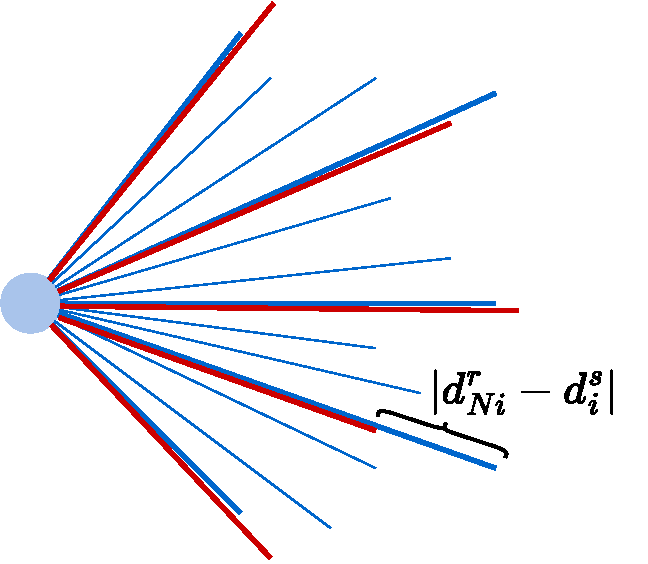
\includegraphics[width=\textwidth]{Figures/MotionPlanning/ParticleFilterLaserComparison.pdf}
      \end{figure}
    \end{column}
    \begin{column}{0.6\textwidth}
      Para obtener una medida de comparación se obtiene una media de diferencias en las distancias:
      \[\delta = \sum_{i=0}^{M_s - 1}\left|d^r_{Ni} - d^s_i\right|\]
      \[s = e^{-\delta^2/\sigma^2}\]
      con:
      \begin{itemize}
      \item $d^r_{Ni}$: es la $(Ni)$-ésima lectura de distancia del sensor real
      \item $d^s_i$: es la $i$-ésima lectura de distancia del sensor simulado (de una partícula)
      \item $\delta$: media de los valores absolutos de las diferencias
      \item $\sigma^2$: Varianza del sensor (medida de incertidumbre)
      \item $s$: medida de similitud entre el sensor real y el sensor simulado
      \item $M_s$: número de distancias en el sensor simulado ($1/N$ del número de distancias en el sensor real). 
      \end{itemize}
      Recuerde que se simularon solo 1 de cada $N$ lecturas del sensor real
    \end{column}
  \end{columns}
\end{frame}

\begin{frame}\frametitle{Remuestreo con reemplazo}
  \begin{itemize}
  \item Las similitudes obtenidas en el paso anterior pueden usarse como distribución de probabilidad si se normalizan para que sumen 1
  \item La distribución de probabilidad anterior determina la probabilidad de que una partícula sea remuestreada
  \item Para evitar tener partículas repetidas, a cada partícula remuestreada se le suma ruido Gaussiano
  \end{itemize}
  \begin{figure}
    \centering
    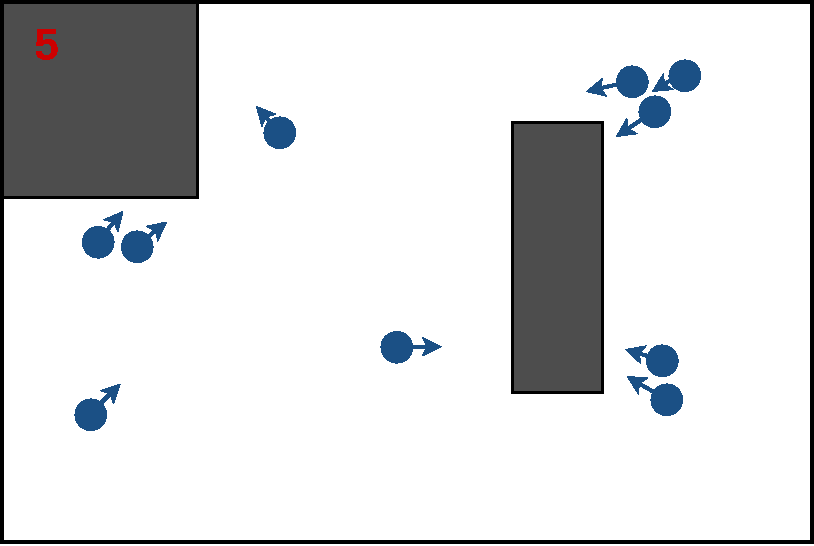
\includegraphics[width=0.35\textwidth]{Figures/MotionPlanning/ParticleFilter5.pdf}
  \end{figure}
\end{frame}

\section{Evasión de obstáculos}
\begin{frame}\frametitle{Evasión de obstáculos}
  \begin{itemize}
  \item Hasta el momento se tiene una manera de representar el ambiente, planear una ruta y seguirla
  \item ¿Qué pasa si en el ambiente hay un obstáculo que no estaba en el mapa?
  \item Se requiere de una técnica reactiva para evadir obstáculos
  \item Una posible solución es el uso de campos potenciales artificiales
  \end{itemize}
\end{frame}

\begin{frame}\frametitle{Campos potenciales artificiales}
  El objetivo de esta técnica es diseñar una función $U(q):\mathbb{R}^n\rightarrow \mathbb{R}$ que represente energía potencial.
  \begin{itemize}
  \item El gradiente $\nabla U(q) = \left[\frac{\partial U}{\partial q_1},\dots,\frac{\partial U}{\partial q_n}\right]$ es una fuerza.
  \item Se debe diseñar de modo que tenga un mínimo global en el punto meta y máximos locales en cada obstáculo.
  \item Si el robot se mueve siempre en sentido contrario al gradiente $\nabla U$ llegará al punto meta siguiendo una ruta alejada de los obstáculos.
  \item Ha varias formas de diseñar la función $U(q)$, algunas son:
    \begin{itemize}
    \item Algoritmo \textit{wavefront}, requiere una discretización del espacio (requiere mapa previo), pero no presenta mínimos locales.
    \item Campos atractivos y repulsivos, no requieren mapa previo, pero pueden presentar mínimos locales. 
    \end{itemize}
  \end{itemize}
\end{frame}

\begin{frame}\frametitle{Potenciales atractivos y repulsivos}
  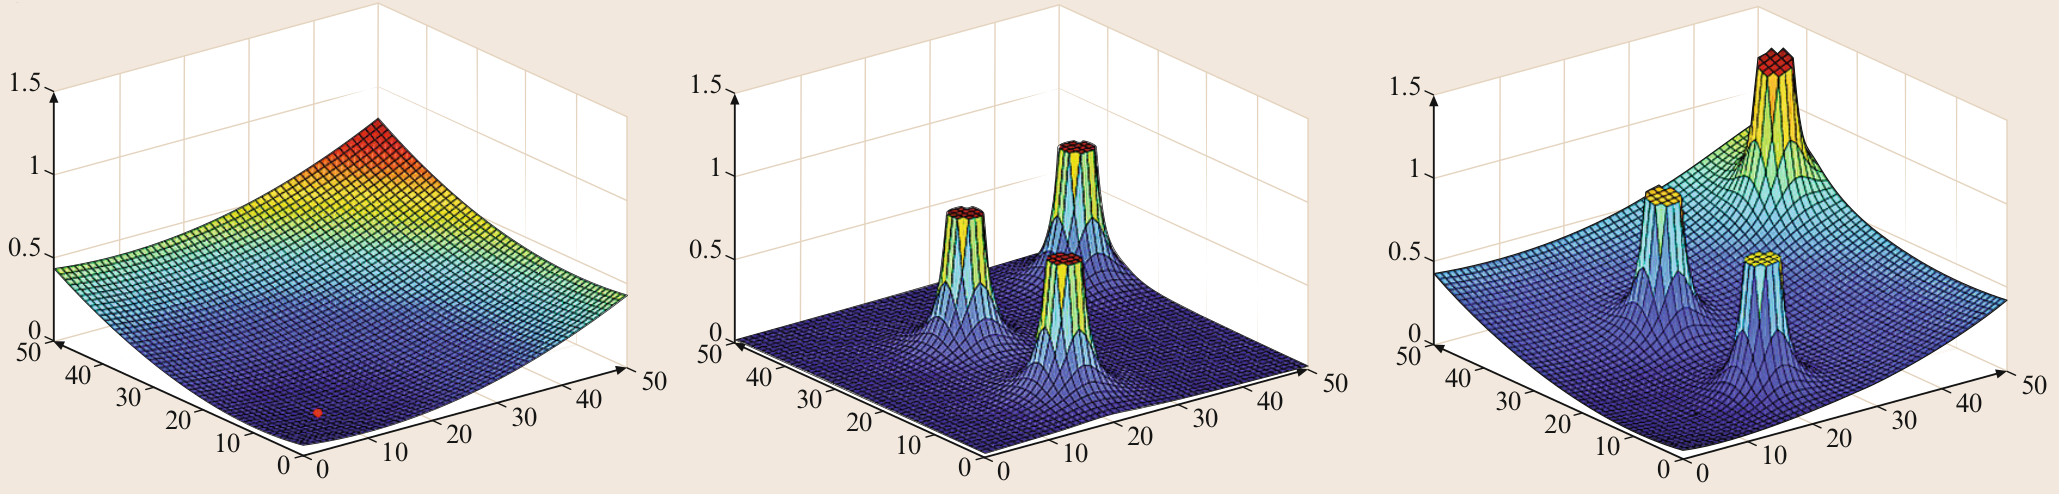
\includegraphics[width=\textwidth]{Figures/MotionPlanning/PotFieldsExample.png}
  \begin{itemize}
  \item \textbf{Campos repulsivos:} Por cada obstáculo se diseña una función $U_{rej_i}(q)$ con un máximo local en la posición $q_{o_i}$ del obstáculo.
  \item \textbf{Campo atractivo:} Se diseña una función $U_{att}(q)$ con un mínimo global en el punto meta $q_g$.
  \item La función potencial total $U(q)$ se calcula como
    \[ U(q) = U_{att}(q) + \frac{1}{N}\sum_{i=1}^N U_{rej_i}(q)\]
  \end{itemize}
\end{frame}

\begin{frame}\frametitle{Fuerzas atractiva y repulsivas}
  Puesto que el gradiente es un operador lineal, se pueden diseñar directamente las fuerzas atractiva $F_{att}(q) = \nabla U_{att}(q)$ y repulsivas $F_{rej_i}(q) = \nabla U_{rej_i}(q)$, de modo que la fuerza total será:
  \[ \nabla U(q) = F(q) = F_{att}(q) + \frac{1}{N}\sum_{i=1}^N F_{rej_i}(q)\]
  Una propuesta de estas fuerzas es:
  \begin{eqnarray*}
    \label{eq:attractive}
    F_{att} &=& \eta \dfrac{\left(q - q_g\right) }{\Vert q - q_g \Vert},\qquad \zeta > 0\label{eq:PotFieldsAttraction}\\
    F_{rej} &=& \begin{cases}
                  \zeta\left(\sqrt{\dfrac{1}{d} - \dfrac{1}{d_0}}\right)\dfrac{q_{o_i} - q}{d}
                  & \quad\textrm{si}\quad d < d_0\\
                  0 & \quad\textrm{en otro caso}
                \end{cases}
  \end{eqnarray*}
  donde
  \begin{itemize}
  \item $q=(x,y)$ es la posición del robot
  \item $q_g=(x_g, y_g)$ es el punto que se desea alcanzar
  \item $q_{o_i} = (x_{o_i}, y_{o_i})$ es la posición del $i$-ésimo obstáculo
  \item $d_0$ es una distancia de influencia. Más allá de $d_0$ los obstáculos no producen efecto alguno
  \item $\zeta$ y $\eta$, junto con $d_0$, son constantes de sintonización
  \end{itemize}
\end{frame}

\begin{frame}\frametitle{Evasión de obstáculos por campos potenciales}
  \begin{itemize}
  \item Aunque las ecuaciones anteriores suponen que se conoce la posición de cada obstáculo $q_{o_i}$, en realidad ésta aparece siempre en la diferencia $q_{o_i} - q$, es decir, solo se requiere su posición relativa al robot.
  \item Los campos potenciales se implementan utilizando el lidar, donde cada lectura se considera un obstáculo. 
  \end{itemize}
  \begin{figure}
    \centering
    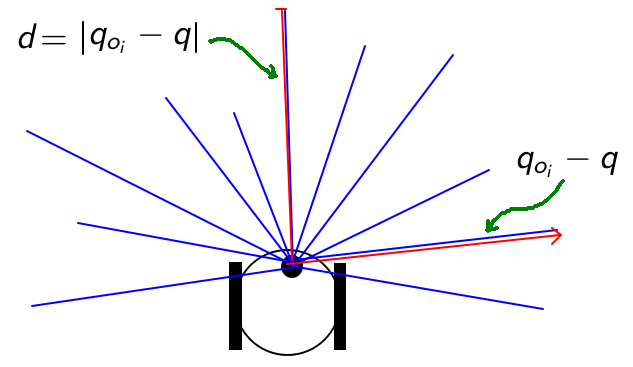
\includegraphics[width=0.4\textwidth]{Figures/MotionPlanning/PotFieldsLidar.png}
  \end{figure}
  Las lecturas del lídar generalmente son pares distancia-ángulo $(d_i,\theta_i)$ expresados con respecto al robot, por lo que, si se conoce la posición del robot $(x_r,y_r,\theta_r)$, la posición de cada obstáculo se puede calcular como:
  \begin{eqnarray*}
    x_{oi} &=& x_r + d_i\cos(\theta_i + \theta_r)\\
    y_{oi} &=& y_r + d_i\sin(\theta_i + \theta_r)\\
  \end{eqnarray*}
\end{frame}

\begin{frame}\frametitle{Evasión de obstáculos por campos potenciales}
  Finalmente, para que el robot alcance el punto de menor potencial, se puede emplear el descenso del gradiente:
  \[\]
  \begin{algorithm}[H]
  \DontPrintSemicolon
  \KwData{Posición inicial $q_s$, posición meta $q_g$, posiciones $q_{oi}$ de los obstáculos y tolerancia $tol$}
  \KwResult{Secuencia de puntos $\{q_0,q_1, q_2, \dots\}$ para evadir obstáculos y alcanzar el punto meta}
  \;
$q \leftarrow q_s$\;
\While{$\Vert\nabla U(q)\Vert > tol$}
{
  $q \leftarrow q - \epsilon F(q)$\;
  $[v,\omega] \leftarrow $ leyes de control con $q$ como posición deseada\;
}
  \caption{Descenso del gradiente para mover al robot a través de un campo potencial.}
  \label{alg:PotFields}
\end{algorithm}
\end{frame}

\begin{frame}\frametitle{Evasión de obstáculos por campos potenciales}
  Ejemplo de movimiento:
  \begin{figure}
    \centering
    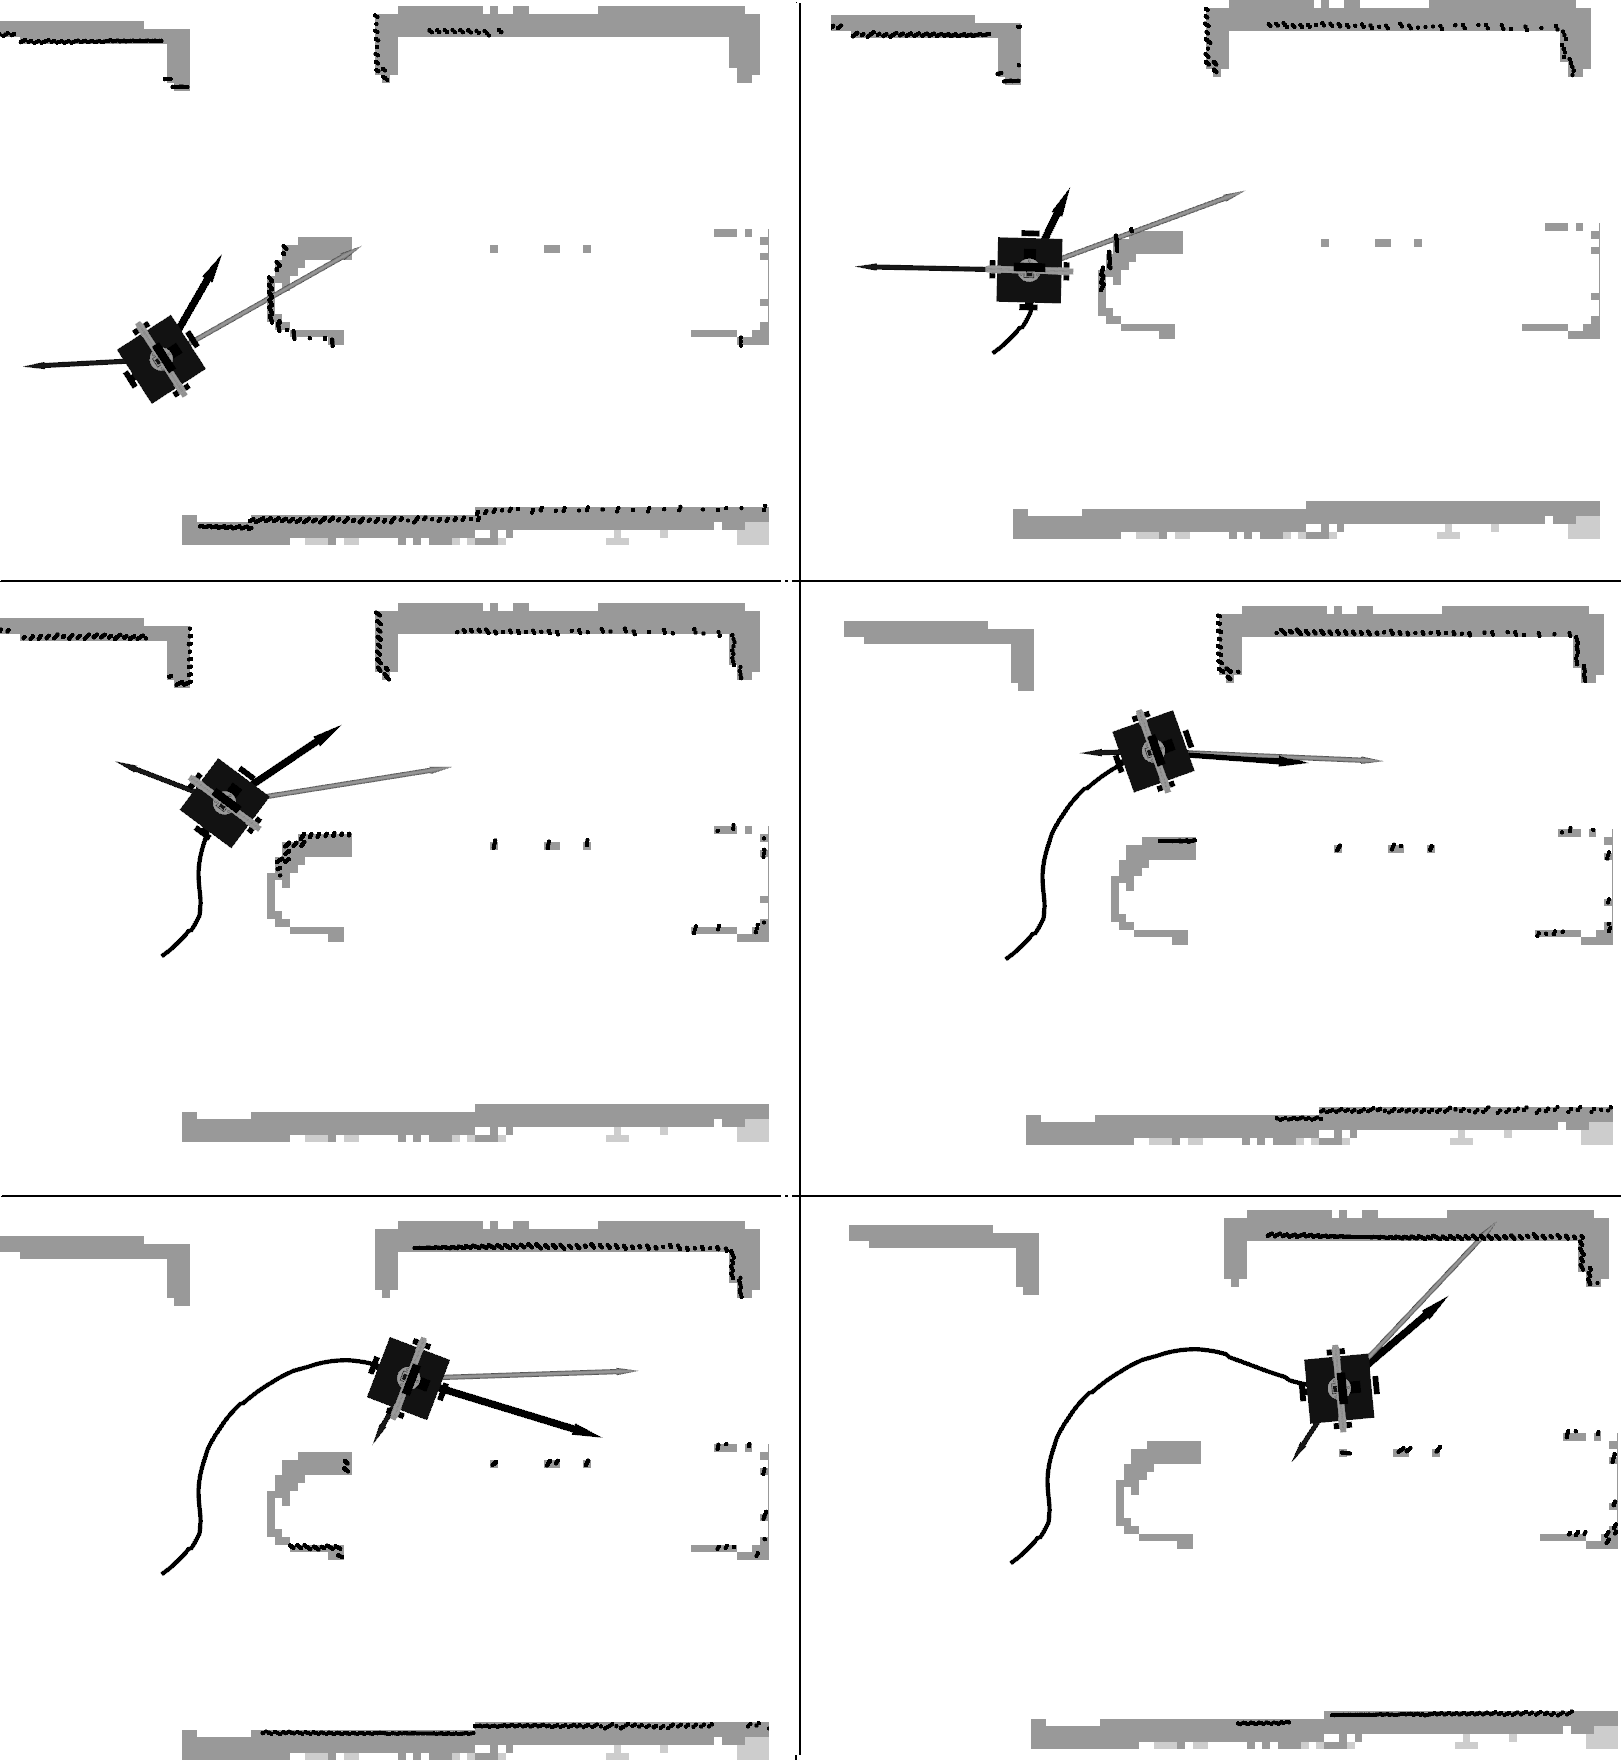
\includegraphics[height=0.85\textheight]{Figures/MotionPlanning/PotFieldsExecution.png}
  \end{figure}
\end{frame}

\begin{frame}\frametitle{Navegación: el enfoque tradicional}
  \begin{columns}
    \begin{column}{0.5\textwidth}
      Mapas geométricos (los más comunes son las celdas de ocupación) para representar el ambiente
      \begin{figure}
        \centering
        \includegraphics[width=0.5\textwidth]{Figures/OccupancyGrid.png}
      \end{figure}
      Planeadores de rutas basados en grafos o basados en muestreo
      \begin{figure}
        \centering
        \includegraphics[width=0.7\textwidth]{Figures/AStarComparison.png}
      \end{figure}
    \end{column}
    \begin{column}{0.5\textwidth}
      Filtros de partículas (también EKF) para localización y mapeo
      \begin{figure}
        \centering
        \includegraphics[width=0.55\textwidth]{Figures/ParticleFilter4.pdf}
      \end{figure}
      Evasión de obstáculos mediante campos potenciales
      \begin{figure}
        \centering
        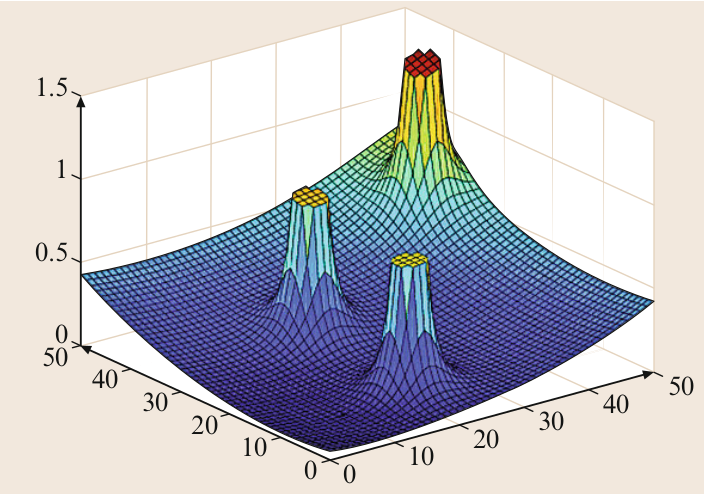
\includegraphics[width=0.55\textwidth]{Figures/PotFields.png}
      \end{figure}
    \end{column}
  \end{columns}
  \textbf{Desventaja:} Se requiere un mapa geométrico. No es posible aprender a navegar y luego usar el conocimiento para nevegar en un ambiente diferente. 
\end{frame}

\begin{frame}\frametitle{Navegación: ¿qué sigue?}
  Navegación sin mapa (geométrico)
  \begin{figure}
    \centering
    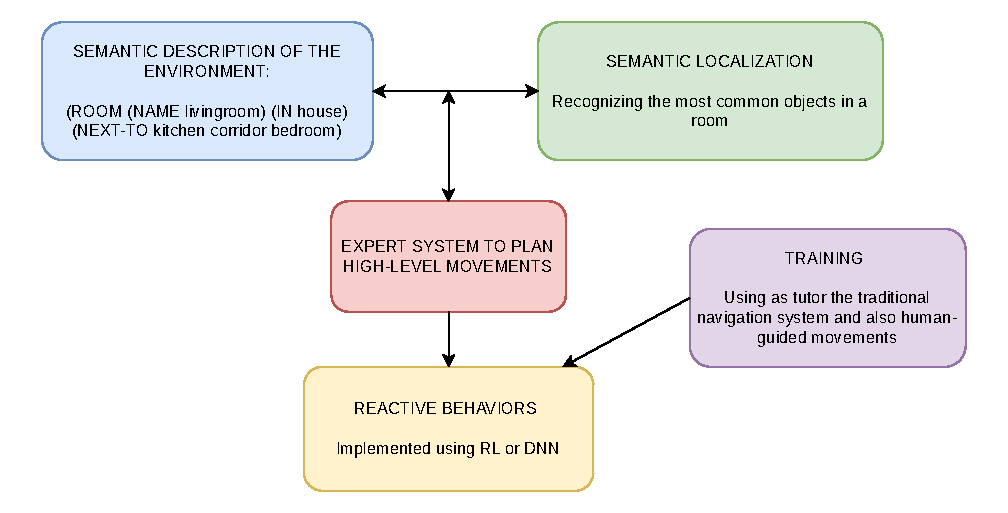
\includegraphics[width=0.8\textwidth]{Figures/MaplessNavigation.pdf}
  \end{figure}
\end{frame}


\begin{frame}\frametitle{Navegación reactiva usando DNN}
  \begin{columns}
    \begin{column}{0.25\textwidth}
      Discretización del espacio alrededor del robot:
      \begin{figure}
        \centering
        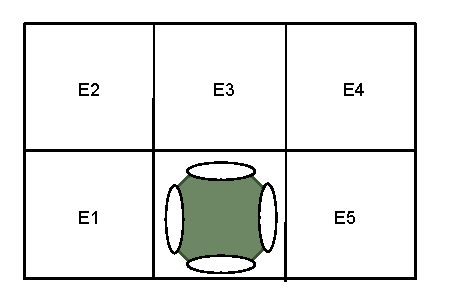
\includegraphics[width=0.8\textwidth]{Figures/RLStates.pdf}
      \end{figure}
      Discretización de los comandos de velocidad como acciones::
      \begin{figure}
        \centering
        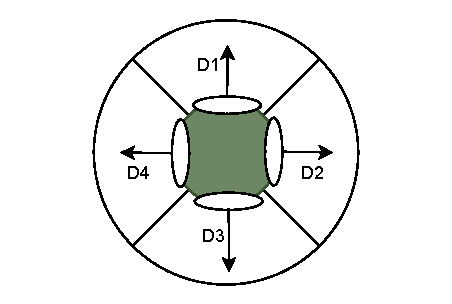
\includegraphics[width=0.8\textwidth]{Figures/RLActions.pdf}
      \end{figure}
    \end{column}
    \begin{column}{0.4\textwidth}
      DNN para generar comandos de velocidad:
      \begin{figure}
        \centering
        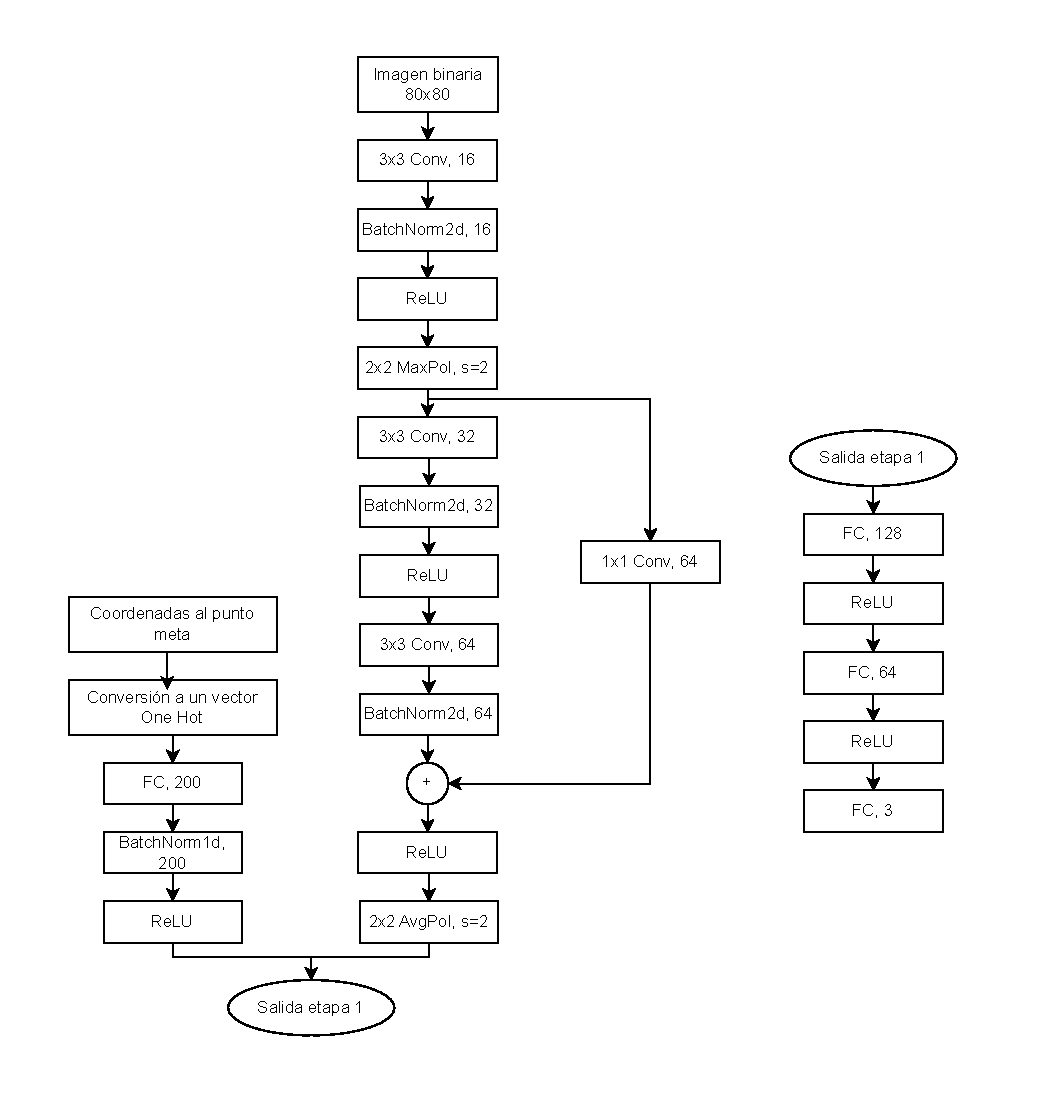
\includegraphics[width=0.95\textwidth]{Figures/DNN.pdf}
      \end{figure}
      Entrenamiento usando datos generados por humanos y datos generados usando campos potenciales
    \end{column}
    \begin{column}{0.35\textwidth}
      Pruebas en ambientes diferentes al de entrenamiento:
      \begin{figure}
        \centering
        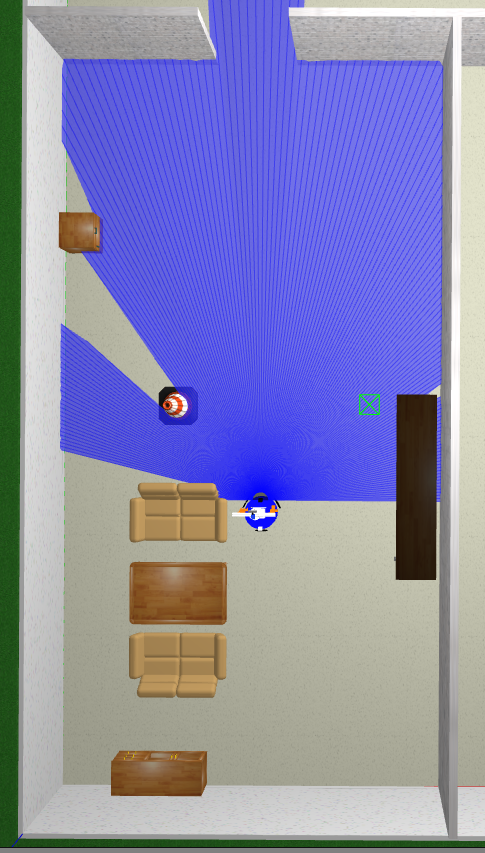
\includegraphics[width=0.45\textwidth]{Figures/Ambiente1.png}
        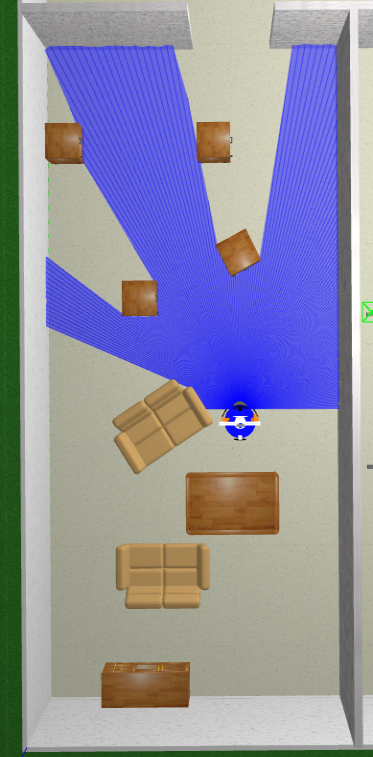
\includegraphics[width=0.45\textwidth]{Figures/Ambiente2.png}
      \end{figure}
      En el ambiente conocido (izq), la navegación basada en grafos y los campos potenciales superaron a las DNN, pero en el ambiente desconocido (derecha), la DNN superó a ambos métodos. 
    \end{column}
  \end{columns}
\end{frame}

\begin{frame}\frametitle{Videos}
  \url{https://youtu.be/ozKxjrrxchI}
\end{frame}


\bibliographystyle{abbrv}
\bibliography{References}
\begin{frame}
  \Large{Contact}
  \[\]
  \large
  Dr. Marco Negrete\\
  Associated Professor\\
  Signal Processing Department\
  School of Engineering, UNAM.
  \[\]
  marco.negrete@ingenieria.unam.edu\\
\end{frame}
\end{document}
